% zip ms_files.zip ms.tex abstract.tex intro.tex method.tex results.tex
% acknowledgments.tex appendix.tex
% conclusion.tex Praesepe.pdf variance.pdf simulated_CMD.pdf
% rotation_model_praesepe.pdf simulation_results.pdf NGC6819.pdf
% NGC6819_results.pdf hz.bib asteroseismic_results_nosdss_gaia.pdf

\documentclass[useAMS, usenatbib, preprint, 12pt]{aastex}
% \documentclass[a4paper,fleqn,usenatbib,useAMS]{mnras}
\usepackage{cite, natbib}
\usepackage{float}
\usepackage{amsmath}
\usepackage{hyperref}
\usepackage{epsfig}
\usepackage{cases}
\usepackage[section]{placeins}
\usepackage{graphicx, subfigure}
\usepackage{color}
\usepackage{bm}

\AtBeginDocument{\let\textlabel\label}

\newcommand{\ie}{{\it i.e.}}
\newcommand{\eg}{{\it e.g.}}
\newcommand{\etal}{{\it et al.}}

\newcommand{\kepler}{{\it Kepler}}
\newcommand{\Kepler}{{\it Kepler}}
\newcommand{\corot}{{\it CoRoT}}
\newcommand{\Ktwo}{{\it K2}}
\newcommand{\ktwo}{\Ktwo}
\newcommand{\TESS}{{\it TESS}}
\newcommand{\tess}{{\it TESS}}
\newcommand{\LSST}{{\it LSST}}
\newcommand{\lsst}{{\it LSST}}
\newcommand{\Wfirst}{{\it WFIRST}}
\newcommand{\wfirst}{{\it WFIRST}}
\newcommand{\SDSS}{{\it SDSS}}
\newcommand{\PLATO}{{\it PLATO}}
\newcommand{\plato}{{\it PLATO}}
\newcommand{\Gaia}{{\it Gaia}}
\newcommand{\gaia}{{\it Gaia}}
\newcommand{\panstarrs}{{\it PanSTARRS}}

\newcommand{\Teff}{$T_{\mathrm{eff}}$}
\newcommand{\teff}{$T_{\mathrm{eff}}$}
\newcommand{\FeH}{[Fe/H]}
\newcommand{\feh}{[Fe/H]}
\newcommand{\prot}{$P_{\mathrm{rot}}$}
\newcommand{\pmega}{$\bar{\pi}$}
\newcommand{\mj}{$m_j$}
\newcommand{\mh}{$m_h$}
\newcommand{\mk}{$m_k$}
\newcommand{\mx}{$m_x$}
\newcommand{\logg}{log(g)}
\newcommand{\dnu}{$\Delta \nu$}
\newcommand{\numax}{$\nu_{\mathrm{max}}$}

% \newcommand{\nsim_stars}{841}

\newcommand{\amnh}{1}
\newcommand{\cca}{2}
\newcommand{\florida}{3}
\newcommand{\hawaii}{4}
\newcommand{\columbia}{5}
\newcommand{\riverside}{6}
\newcommand{\cuny}{7}
\newcommand{\nyu}{8}
\newcommand{\cds}{9}
\newcommand{\mpia}{10}
\newcommand{\yale}{11}

\newcommand{\sd}{{\tt stardate}}
\newcommand{\MS}{main sequence}
\newcommand{\ms}{main sequence}
\newcommand{\Ms}{Main sequence}
\newcommand{\gcolor}{$G_{BP} - G_{RP}$}
\newcommand{\fhat}{$\hat{F}$}
\newcommand{\cbv}{$C_{B-V}$}
\newcommand{\eep}{equivalent evolutionary point}
\newcommand{\Eep}{Equivalent evolutionary point}

% \newcommand{\racomment}[1]{{\color{blue}#1}}
\newcommand{\racomment}[1]{{\bf #1}}

\begin{document}

% \title{Inferring stellar ages by combining isochrone fitting with
% gyrochronology}
% \title{A new age-dating model for cool main sequence stars that combines
% isochrone fitting with gyrochronology}
\title{Towards precise stellar ages: combining isochrone fitting with
empirical gyrochronology}

\author{%
    Ruth Angus\altaffilmark{\amnh, }\altaffilmark{\cca, },
    Timothy D. Morton\altaffilmark{\florida, }\altaffilmark{\cca, },
    Daniel Foreman-Mackey\altaffilmark{\cca},
    Jennifer van Saders\altaffilmark{\hawaii},
    Jason Curtis\altaffilmark{\columbia},
    Stephen R. Kane\altaffilmark{\riverside},
    Megan Bedell\altaffilmark{\cca},
    Rocio Kiman\altaffilmark{\cuny, }\altaffilmark{\amnh},
    David W. Hogg\altaffilmark{\nyu, }\altaffilmark{\cca,
}\altaffilmark{\cds, }\altaffilmark{\mpia},
    John Brewer\altaffilmark{\yale}
}

\altaffiltext{\amnh}{American Museum of Natural History, Central Park West,
Manhattan, NY, USA}
\altaffiltext{\cca}{Center for Computational Astrophysics, Flatiron Institute,
162 5th Avenue, Manhattan, NY, USA}
\altaffiltext{\florida}{Department of Astronomy, University of Florida,
Gainesville, FL, USA}
\altaffiltext{\hawaii}{Institute for Astronomy, University of Hawai'i at
M\={a}noa, Honolulu, HI, USA}
\altaffiltext{\columbia}{Department of Astronomy, Columbia
University, Manhattan, NY, USA}
\altaffiltext{\riverside}{
Department of Earth and Planetary Sciences, University of California,
Riverside, CA 92521, USA}
\altaffiltext{\cuny}{Department of physics, CUNY Graduate Center, City
University of New York, Manhattan, NY, USA}
\altaffiltext{\nyu}{Center for Cosmology and Particle Physics, New York
University, Manhattan, NY, USA}
\altaffiltext{\cds}{Center Data Science, New York
University, Manhattan, NY, USA}
\altaffiltext{\mpia}{Max-Planck Institute for Astronomy,
K{\"o}nigstuhl, Heidelberg, Germany}
\altaffiltext{\yale}{Yale center for astronomy and astrophysics, Yale
University, New Haven, CT, USA}

\begin{abstract}
We present a new age-dating technique that combines gyrochronology and
isochrone fitting to infer ages for FGKM main-sequence and subgiant field
stars.
The age-dating methods of gyrochronology and isochrone fitting are each
capable of providing relatively precise ages in certain areas of the
Hertzsprung-Russell diagram: rotation periods can provide precise ages for
cool stars on the main sequence via gyrochronology, and isochrone fitting
can provide precise ages for stars near the main-sequence turnoff.
Combined, these two age-dating techniques can be applied to a broader range of
stellar masses and evolutionary stages and can provide ages that are more
precise and accurate than either method used in isolation.
In this investigation, we demonstrate that the position of a star on the
Hertzsprung-Russell or color-magnitude diagram can be combined with its
rotation period to infer a precise age via both isochrone fitting and
gyrochronology simultaneously.
We show that incorporating rotation periods with 5\% uncertainties into
stellar evolution models particularly improves age precision for FGK stars on
the main sequence, and can, on average, provide age estimates that are up to
three times more precise than isochrone fitting alone for these stars.
In addition, we provide a new gyrochronology relation, calibrated to the
Praesepe cluster and the Sun, that includes a variance model to capture the
rotational behavior of stars whose rotation periods do not lengthen with the
square-root of time, and parts of the Hertzsprung-Russell diagram where
gyrochronology has not been calibrated.
This publication is accompanied by an open source {\it Python} package (\sd:
\url{ https://github.com/ruthangus/stardate }) for inferring the ages of main
sequence and subgiant FGKM stars from rotation periods, spectroscopic
parameters and/or apparent magnitudes and parallaxes.
\end{abstract}

\section{Introduction}
\label{section:intro}

Age is the most difficult stellar property to measure, and the difficulty of
age-dating is particularly acute for low mass (GKM) stars on the main sequence
(MS).
Using conventional dating methods, uncertainties on the ages of these stars
can be as large as the age of the Universe.
GKM dwarfs are difficult to age-date because most of their physical and
observable properties do not change rapidly.
This is represented in the spacing of isochrones on a Hertzsprung-Russell
diagram (HRD) or color-magnitude diagram (CMD).
On the MS, isochrones are tightly spaced and, even with very precise
measurements of effective temperature and luminosity, the position of a MS
star on the HRD may be consistent with range of isochrones spanning several
billion years.
At the main-sequence turnoff however, isochrones are spread further apart, so
that sufficiently precisely measured temperatures and luminosities can yield
ages that are extremely precise (with minimum statistical uncertainties on the
order of 5-10\%) \citep[\eg][]{pont2004}.
% Typical age uncertainties of dwarfs.
The classical method for measuring stellar ages is isochrone placement, or
isochrone fitting, where surface gravity changes resulting from fusion in the
core (usually observed via luminosity, $L$, and effective temperature, \teff,
or absolute magnitude and colour) are compared with a set of models that trace
stellar evolution across the HRD, or CMD.
CMD/HRD position has been thoroughly mapped with physical models, and can be
used to calculate relatively accurate (but not necessarily precise) ages,
barring some systematic variations between different models,
\citep[\eg][]{yi2001, dotter2008, dotter2016}.
On the MS itself, there is little differentiation between stars of different
ages in the $L$ and \teff\ plane, so ages tend to be very imprecise.
The method of inferring a star's age from its rotation period, called
`gyrochronology', is much better suited for measuring ages on the MS because
MS stars spin down relatively rapidly.

Magnetic braking in MS stars was first observed by \citet{skumanich1972} who,
studying young clusters and the Sun, found that the rotation periods of
Solar-type stars decay with the square-root of time.
It has since been established that the rotation period of a MS star depends,
to first order, only on its age and effective temperature or color
\citep[\eg][]{barnes2003}.
The convenient characteristic of stars that allows their ages to be inferred
from their {\it current} rotation periods and independently of their
primordial ones, comes from the steep dependence of spin-down rate on rotation
period \citep{kawaler1989}.
Stars spinning with high angular velocity will experience a much greater
angular momentum loss rate than slowly spinning stars and for this reason, no
matter the initial rotation period, Solar type stars will have the same
rotation period after around the age of the Hyades, 500-700 million years
\citep{irwin2009, gallet2015}.
After this time, the age of a star can be inferred, to first order, from its
dust-corrected color (\eg\ B-V or \gcolor) and {\it current} rotation period
alone \citep[See][for an analysis of how initial conditions effect gyrochronal
ages]{epstein2014}.

The relation between age, rotation period and mass has been studied in detail,
and several different models have been developed to capture the rotational
evolution of Sun-like stars.
Some of these models are theoretical and based on physical processes; modeling
angular momentum loss as a function of stellar properties as well as the
properties of the magnetic field and stellar wind \citep[\eg][]{kawaler1988,
kawaler1989, pinsonneault1989, vansaders2013, matt2015, vansaders2016}.
Other models are empirical and capture the behavior of stars from a purely
observational standpoint, using simple functional forms that can reproduce the
data \citep[\eg][]{barnes2003, barnes2007, mamajek2008, angus2015}.
Both types of model, theoretical and empirical, must be calibrated using
observations.
Old calibrators are especially important because new evidence suggests that
rotational evolution goes through a transition at old age or, more
specifically, at a large Rossby number, $Ro$ (the ratio of rotation period to
the convective overturn timescale).
For example, stars shown to be old from \kepler\ asteroseismic data rotate
more rapidly than expected given their age \citep{angus2015, vansaders2016}.
A new physically motivated gyrochronology model, capable of reproducing these
data, was recently introduced \citep{vansaders2016}.
It relaxes magnetic braking at a critical Rossby number of around 2,
approximately the Solar value.
This model predicts that, after stellar rotation periods lengthen enough to
move stars across this $Ro$ threshold, stars conserve angular momentum and
maintain a nearly constant rotation period from then until they evolve off the
MS.
% As demonstrated in section \ref{section:results} however, this does not mean
% that the ages of stars with Ro $>$ 2 cannot be measured from their rotation
% periods, especially if their rotation periods are combined with HRD or CMD
% placement.

The gyrochronology models that capture post $Ro$-threshold, rotational
evolution \citep{vansaders2016} are the current state-of-the-art in rotation
dating.
These models can be computed over a grid of stellar parameters, and
interpolated-over to predict the age of a star.
The process of measuring the age of a field star with these models is similar
to inferring an age using any set of isochrones, with the difference being
that rotation period is an additional observable dimension.
Ages calculated using these models are therefore likely to be much more
precise than using rotation-free isochrones since rotation period provides an
additional anchor-point for the age of a star.
We present here a complementary method that combines isochrones with an {\it
empirical} gyrochronology model.
The methodology is related to the \citet{vansaders2016} model in that both use
a combination of rotation periods and other observable properties that track
stellar evolution on the HRD in concert.
The main difference is that the gyrochronology model used here is an entirely
empirically calibrated one, as opposed to a physically derived one.

One major advantage of using a physically motivated gyrochronology model is
the ability to rely on physics to interpolate or extrapolate over parts of
parameter space with sparse data coverage.
However, rotational spin-down is a complex process that is not yet fully
understood and currently no physical model can accurately reproduce all the
data available.
For this reason, even physically motivated gyrochronology models cannot always
be used to reliably extrapolate into unexplored parameter space.
Physical models, when calibrated to data, can provide insight into the physics
of stars, however, if accurate and precise {\it prediction} of stellar
properties is desired, empirical models can have advantages over physical
ones.
For example, the data may reveal complex trends that cannot be reproduced with
our current understanding of the physical processes involved, but may be
captured by more flexible data-driven models.
In addition, it is relatively straightforward to build an element of
stochasticity into empirical models, \ie\ to allow for and incorporate
outliers or noisy trends.
This is particularly important for stellar spin down because rotation periods
can be affected by additional confounding variables which are not always
observed (having a binary or planetary companion, for example).
A further advantage of empirical models is that inference is more tractable:
it can be extremely fast to fit them to data.

In this work we calibrated a new empirical gyrochronology relation, fit to the
Praesepe open cluster and the Sun, in \gaia\ \gcolor\ color.
\Gaia\ $G$, $G_{BP}$ and $G_{RP}$ apparent magnitudes are now the most
abundant photometric measurements, available for more than a billion stars
\citep{brown2018}.
In fact, an important point of context for this work is the new
availability of data relevant to gyrochronology and stellar ages.
\Gaia\ now provides broad-band photometry and parallaxes for over a billion
stars, and \kepler, \ktwo\ and \tess\ are providing rotation periods for
hundreds of thousands of stars.
Gyrochronology is becoming one of the most readily available age-dating
methods, so continuing to improve gyrochronology relations and methods is
important.
Like any other gyrochronology relation, this new Praesepe-based model does not
perfectly reproduce all the observed data and some simple modifications could
make significant improvements, for example, by including a mixture model to
account for outliers and binaries, and by removing the period-age,
period-color separability to account for different period-color shapes seen in
clusters of different ages.
We leave these improvements for a future project and, for now, test this
new Praesepe-based model, which is built into an open source {\it Python}
package for gyrochronology called \sd.
\sd\ provides the framework for simultaneous gyrochronology and isochrone
fitting, and, because \sd\ is modular, it would be straightforward to update
the gyrochronology relation in the future.

This paper is laid out as follows.
In section \ref{section:method} we describe our new age-dating model and its
implementation, in section \ref{section:results} we test this model on
simulated stars and cluster stars, and in section \ref{section:conclusion} we
discuss the implications of these tests and future pathways for development.
Throughout this paper we use the term {\it `observables'} to refer to the
following observed properties of a star: \teff, \logg, observed bulk
metallicity ($[\mathrm{Fe/H}]$), parallax ($\bar{\pi}$), photometric
colors in different passbands (${\bf m_x} = [m_J, m_H, m_K, m_B, m_V, m_G,
m_{GBP}, m_{GRP}...]$, etc) and rotation period ($P_{\mathrm{rot}}$).
The term `parameters' refers to the physical properties of that star: age
($t$), equivalent evolutionary phase (EEP), model metallicity
($\mathrm{M/H}$), distance ($D$) and V-band extinction ($A_V$).
These are the properties that generate the observables.

% \section{Combining isochrone fitting with Gyrochronology: Motivation}
\label{section:motivation}

In order to demonstrate why a combination of gyrochronology and isochrone
fitting can provide more precise ages than either method used in isolation, we
calculated the information provided by each method for a range of stellar
masses, ages and evolutionary stages.

According to observations of cluster stars and the Sun, the decrease in
rotation period with time is roughly proportional to the inverse square root
of age, $\frac{dP_{\mathrm{rot}}}{dt} \propto \mathrm{Age}^{-n}$, where
n$\sim$0.5.
This corresponds to a large rate of change relative to typical rotation
period measurement uncertainties.
For example, the Sun's rotation period is currently decreasing at a rate of
around 3 days per billion years \citep[unless it has already stopped spinning
down, \eg][]{vansaders2016}, and the 1 billion year-old Sun
spun down at a rate of around 6 days per billion years.
These are relatively large changes compared with the average uncertainties on
rotation period measurements: the median rotation period uncertainty in the
\citet{mcquillan2014} catalog is around 0.1 days.
In contrast, the temperature of a K dwarf changes by about 20 K every billion
years which is small compared to typical observational uncertainties of 20-100
K.
Rotational isochrones, or `gyrochrones' provide much more {\it information}
about age than traditional isochrones.
The difference in information conveyed by rotation vs \teff\ and $L$ can be
quantified by calculating the time derivatives of a star's observables.
The rate of change of \teff\ and $L$ dictates the minimum theoretically
achievable uncertainty on an age inferred via isochrone fitting, given some
observational uncertainties.
Similarly, the rate of change of rotation period dictates the minimum
achievable uncertainty on an age inferred via gyrochronology.
In order to quantify the minimum theoretical uncertainty on ages calculated
via isochrone fitting and gyrochronology, we calculated the Fisher information
for the MIST isochrones \citep{paxton2011, paxton2013, paxton2015, dotter2016,
choi2016, paxton2018} and an empirical polynomial gyrochronology model we fit
to the Praesepe cluster.
The Fisher information quantifies the amount of information that an observable
imparts onto an unknown parameter.
In the case of isochrone fitting on a CMD using \Gaia\ data, the observables
are \Gaia\ absolute magnitude $M_G$ and color, \gcolor\ and the parameter is
age, or time, $t$.
The Fisher information is the variance of the parameter, $t$, given the
covariance of the observables and their derivatives with respect to $t$.
The inverse covariance matrix of the parameters (in this case we have just one
parameter, age or time, $t$), given the covariance matrix of the data,
${\bf y} = [M_G, G_{BP} - G_{RP}]$, is given by the following equation,
\begin{equation}
    C_{\mathrm{Age}}^{-1} = \left[\frac{d{\bf y}}{dt}\right]^T
    C_{\bf y}^{-1} \left[\frac{d{\bf y}}{dt}\right].
\end{equation}
Since we just have one parameter, $C_\mathrm{Age}^{-1}$ is a scalar, the
inverse variance of age, $\sigma_{\mathrm{Age}}^{-2}$.
In order to calculate the age uncertainty from the MIST isochrones, we
calculated numerical derivatives of $\frac{dG}{dt}$,
and $\frac{d(G_{BP} - G_{RP})}{dt}$ at every point on the MIST model grids.
We then calculated the isochronal age uncertainty, $\sigma_{\mathrm{Age}}$ at
every point on the grid.
Figure \ref{fig:iso_fisher} shows Solar-metallicity MIST isochrones, colored
by $\sigma_{\mathrm{Age}}$.

Figure \ref{fig:iso_fisher}\footnote{Figures \ref{fig:iso_fisher} and
\ref{fig:gyro_fisher} were generated in a {\it Jupyter} notebook available at
the following url:
\url{https://github.com/RuthAngus/stardate/blob/master/paper/code/Fisher_information.ipynb}}
shows the minimum theoretical absolute age uncertainty,
$\sigma_{\mathrm{Age}}$ (left panel), calculated using typical uncertainties
on \Gaia\ absolute magnitude, $M_G$, of $\pm$0.05 and a color spread of 0.05
that (conservatively) accounts for scatter induced by metallicities ranging
from -0.25 to +0.25 dex.
These uncertainties are represented as black errorbars in the top right
corner.
The typical \Gaia\ uncertainties are $0.5$ in both $M_G$ and \gcolor.
These estimates are based on a calculation of the median uncertainty on \Gaia\
absolute G-magnitude of cool stars which is dominated by the parallax
uncertainty.
We assumed the same uncertainty on \gcolor.
The minimum uncertainty on isochronal age ranges from around 10 million years
at MS turn off (upper left yellow area) to around the age of the Universe for
K dwarfs (middle to lower-right blue area).
The minimum {\it relative} age uncertainty,
$\sigma_{\mathrm{Age}}/\mathrm{Age} \times 100$, plotted in the right-hand
panel ranges from less than 1\% for old MS turn off stars with ages
around 13 Gyr and age uncertainties less than 0.1 Gyr, up to tens-of-thousands
of percent for the youngest K and M dwarfs with unconstrained ages.

We also calculated the Fisher information for a {\it combined isochronal and
gyrochronology model.}
In this case we effectively had four observables: $M_G$ and \gcolor,
determined by the MIST isochrones; and $P_{\mathrm{rot}}$ (rotation period)
and \gcolor\ {\it again}, this time determined by the gyrochronology model.
We used a simple gyrochronology model, calibrated by fitting a fourth-order
polynomial in rotation period-\Gaia\ color space and a first order polynomical
in rotation period-age space to the 650 Myr Praesepe cluster and the Sun,
only.
This model is described in more detail later in this section.
We calculated analytic derivatives for $\frac{dP_{\mathrm{rot}}}{dt}$ and
$\left(\frac{d(G_{BP} - G_{RP})}{dt}\right)_{\mathrm{gyro}}$ and combined
these with the numerical derivatives of $\frac{dG}{dt}$ and
$\left(\frac{d(G_{BP} - G_{RP})}{dt}\right)_{\mathrm{iso}}$ in order to
calculate the total age uncertainty, $\sigma_{\mathrm{Age~(iso~\&~gyro)}}$.
Figure \ref{fig:gyro_fisher} shows Solar-metallicity MIST isochrones, colored
by $\sigma_{\mathrm{Age~(iso~\&~gyro)}}$.
The results are presented the same way as figure \ref{fig:iso_fisher} however,
figure \ref{fig:gyro_fisher} shows age uncertainties calculated using
isochrones {\it and a polynomial gyrochronology model}.
The age uncertainties were calculated using typical \Gaia\ $M_G$ and \gcolor\
uncertainties, represented as black errorbars in the top right corner, and
rotation period uncertainties of 1 day.
The minimum theoretical absolute age uncertainty inferred using gyrochronology
and isochrone fitting simultaneously, $\sigma_{\mathrm{Age~(iso~\&~gyro)}}$
(left panel of figure \ref{fig:gyro_fisher}), ranges from tens of millions of
years for stars at MS turn off to a few billion years (up to around 3 Gyr for
old G dwarfs).
The very precise ages at MS turn off are still provided by isochrone fitting
-- the incredible precision achievable with isochrone fitting at MS turn off
dominates over the precision provided by gyrochronology.
On the MS however, gyrochronology provides extremely precise ages and its
precision dominates over isochrone fitting.
The gyrochronology model used to calculate the Fisher information is not
appropriate for stars turning off the MS as it does not account for a rapid
decrease in rotation period that may be caused by the stellar radius
increasing \citep[see][]{vansaders2013}.
% However, it provides an upper limit on $\sigma_{\mathrm{Age,~gyro}}$ which is
% is, in any case, dominated by $\sigma_{\mathrm{Age,~iso}}$.
The right-hand panel of figure \ref{fig:gyro_fisher} shows the {\it relative}
age uncertainty achievable with joint isochronal and gyrochronal age
inference.
Relative age uncertainty,
$\mathrm{Age}/\sigma_{\mathrm{Age~(iso~\&~gyro)}}\times 100$ ranges from less
than 1\% at MS turn off, where isochrones provide precise ages because they
are widely spaced, to a maximum of around 30\% for young G dwarfs, where
gyrochrones are at their most tightly spaced.
The dramatic improvement in age precision seen across the MS when
gyrochronology is used provides the motivation for combining isochrone fitting
with gyrochronology.
The minimum relative age uncertainty for GKM stars on the MS is typically
around 20\% -- gyrochronology predicts precise ages for these kinds of stars.
20\% age precision for gyrochronology was also predicted in previous studies.
\citep{epstein2014}.
Gyrochronology and isochrone fitting are extremely complementary:
gyrochronology contributes most of the precision on the MS because rotation
period information dominates over color and luminosity information, however
it is not applicable to hot stars without deep convection zones
and evolved stars.
These are precisely the stars optimally fitted with isochrone models.
\cocomment{This analysis does raise a question however.
Combining two independent dating methods is useful when both are contributing
information, \ie\ near MS turn off, however given that isochrone fitting
provides so little information on the MS, is there any point in including it
there at all?
Why not just abandon isochrone fitting and use gyrochronology exclusively?
Although isochrones and stellar evolution tracks do not provide precise ages
for MS stars, they do provide {\it masses}, and mass is essential for
obtaining a precise gyrochronal age.
Conversely, gyrochronology can actually enhance mass measurements too by
providing a tighter age constraint: since mass and age are weakly correlated,
this results in a tighter mass constraint.
There are other good reasons to model stars with both isochrones and
gyrochronology on the MS.
Firstly, gyrochronology is not applicable to hot stars \citep[\teff $\gtrsim$
6250,][]{kraft1967} or evolved stars but it is not possible to know whether a
star is evolved, or hot and not just reddened, without modelling it.
Modelling stars with isochrones/stellar evolution tracks is required in order
to know whether gyrochronology is applicable or not.
Secondly, most gyrochronology models are calibrated to either $B-V$ color
(most commonly) or mass.
Mass is usually not directly observable, so must be inferred via modelsj and
$B-V$ is {\it also} not directly observed for every star.
For example, the most widely available colors are now \gaia\ \gcolor\ colors,
and most \Gaia\ stars do not have $B-V$ colors.
In order to calculate gyrochronal ages for stars with {\it any} apparent
magnitudes, not just $B-V$, it is necessary to model stars with isochrones and
gyrochronology simultaneously.}

An important caveat of this demonstration is that this is the minimum
theoretical precision given the {\it adopted} gyrochronology model and, since
the model used for this calculation does not include intrinsic scatter (which
is particularly large for young stars), these minimum age uncertainty
calculations are over-optimistic, especially for young stars.
Similarly, our model does not account for weakened magnetic braking at old
ages \citep{vansaders2016} so is also optimistic for old dwarfs.
Still, figures \ref{fig:iso_fisher} and \ref{fig:gyro_fisher} provide an idea
of the improvement provided by gyrochronology over isochrone fitting alone.
% The Praesepe model

In order to calculate analytic derivatives of the gyrochronology model, we
fit a linear model to the Praesepe open cluster and the Sun (see figure
\ref{fig:praesepe}.
We used a three-dimensional polynomial model to predict age as a
function of \gaia\ color and rotation period for Praesepe and the Sun.
This model consists of a 4th order polynomial in logarithmic Gaia color:
\gcolor, which we write as $C_G$ for simplicity, and a 1st order polynomial (a
straight line) in logarithmic age.
For this analysis, rotation periods for Praesepe were obtained from
\citet{douglas2017} and their \gaia\ colors were obtained by crossmatching
their sky-projected positions with the \gaia\ DR2 catalog.
% We used \gcolor\ instead of (B-V) because, due to the $\sim$ billion stars
% observed by \gaia, it is now the most abundant and widely available
% photometric color.
% Our gyrochronology likelihood function is designed to compare observed
% rotation period to predicted rotation period.
% For this reason the gyrochronology model we used must predict rotation period
% as a function of age and color.
When fitting this gyrochronology model, we chose to make {\it age} the
dependent variable because the uncertainties on stellar age are much greater
than the uncertainties on rotation period.
We fit the following model to Praesepe members:
\begin{equation}
    \log_{10}(A) = a + b\log_{10}(C_G) + c\log_{10}^2(C_G) +
    d\log_{10}^3(C_G) + e\log_{10}^4(C_G) + f\log_{10}(P)
\label{eqn:gyro_age_praesepe}
\end{equation}
where $P$ is rotation period in days, $C_G$ is Gaia color, $A$ is stellar age
in years and the lower case letters are free parameters.
We adopted an age for Praesepe of 650 $\pm$ 100 million years
\citep{fossati2008, gossage2018}, a Solar age of 4.56 $\pm$ 0.01 Gyr
\citep{connelly2012}, and a Solar rotation period of 26 days \citep[][Morris
\etal, in prep]{balthasar1986, howe2000}.
The Sun's color in the Gaia color is 0.82 \citep{casagrande2018}.
We found best-fit values: $a = 7.37 \pm 0.03,~b = -1.4 \pm 0.1,~c = 5.0 \pm
0.8,~d = -34 \pm 3,~e = 66 \pm 14$, and $f = 1.49 \pm 0.02$.
This model and the data it was fit to are plotted in figure
\ref{fig:praesepe}.
To be clear, this model was only used to calculate the Fisher information and
produce figures \ref{fig:iso_fisher} and \ref{fig:gyro_fisher}, because it has
simple analytic derivatives.
Since it was only fit to a single cluster and the Sun it is not generally
applicable and was not used in any other aspects of the analysis performed in
this paper.
The gyrochronology model used throughout the rest of the analysis is described
in section \ref{section:method} and equation \ref{eqn:gyro}.
% The $f$ parameter is the inverse of the slope of the rotation period and age
% which was originally measured to be around 0.5.
% Our Praesepe and Sun-only fit results in a slightly steeper age dependence of
% around 0.67, however this value is likely be
% We inverted this relation to predict rotation period as a function of color
% and age,
% \begin{equation}
%     \log_{10}(P) = \frac{\log_{10}(A) - a - b\log_{10}(C_G) - c\log_{10}^2(C_G) -
%     d\log_{10}^3(C_G) - e\log_{10}^4(C_G)}{f}.
% \label{eqn:gyro_age_praesepe}
% \end{equation}
% Both gyrochronology models of equations \ref{eqn:gyro} and
% \ref{eqn:gyro_age_praesepe} are used to predict the ages of individual
% Praesepe stars from their rotation periods and apparent magnitudes in section
% \ref{section:results}.


\begin{figure}
  \caption{
    This figure shows Solar-metallicity MIST isochrones in \Gaia\ absolute
    G-band magnitude and Gaia $G_{BP} - G_{RP}$ color.
    In the left panel the isochrones are colored by the minimum absolute age
    uncertainty at each point on the CMD, calculated using the Fisher
    information.
    This calculation is based on the typical uncertainties of
    \Gaia\ $G$-band photometry, and a color spread that covers metallicities
    ranging from -0.25 to 0.25 dex (represented by black errorbars in the
    upper right).
    The Sun's position \citep{casagrande2018} is indicated with the Solar\
    symbol.
    The purple color in the top left corresponds to small age uncertainties,
    \ie\ good age precision.
    Age precision increases as stars begin to turn off the MS.
    On the MS however, particularly at low masses, the age precision is poor.
    For late K dwarfs, for example, isochrone fitting age uncertainties exceed
    the age of the Universe.
    This makes sense when you consider that typical \Gaia\ uncertaintes on $G$
    and $G_{BP} - G_{RP}$ exceed the entire width of the MS, which spans
    0.01-14 Gyrs.
    Isochrone fitting is not an appropriate age-dating method for MS stars,
    especially at low masses.
    In the right panel the isochrones are colored by the logarithmic
    {\it relative} age precision at each point in the CMD.
    Relative age uncertainties range from 100\% for the oldest MS GKM stars,
    to several thousand percent for the youngest.
    These age uncertainties were calculated using the derivatives of $G$ and
    $G_{BP} - G_{RP}$ with age, \ie\ the rate of change in a star's luminosity
    and temperature.
    For example, K dwarf temperatures increase at a rate of only around 20 K
    per billion years.
    The precision with which an age can be measured is related to the
    separation between isochrones, which indicate epochs of rapid change
    (steep gradients).
    This figure was created using the following Jupyter notebook:
    \url{https://github.com/RuthAngus/stardate/blob/master/paper/code/Fisher_information.ipynb}
    \label{fig:fischer_iso}
}
  \centering
    \includegraphics[width=1\textwidth]{iso_fisher.pdf}
\label{fig:iso_fisher}
\end{figure}

\begin{figure}
  \caption{
    As figure \ref{fig:iso_fisher}, however in this case the minimum age
    uncertainties are calculated based on isochrone fitting and gyrochronology
    {\it combined}.
    The isochrones are colored by the minimum relative age uncertainty at each
    point on the CMD, calculated using the Fisher information.
    This calculation is based on the typical uncertainties of
    \Gaia\ $G$-band photometry, a color spread that covers metallicities
    ranging from -0.25 to 0.25 dex (represented by black errorbars in the
    upper right), and Kepler rotation period uncertainties (conservatively
    estimated at around 1 day).
    In contrast to figure \ref{fig:iso_fisher}, here the left panel shows the
    {\it logarithmic} absolute age and the right panel shows the linear
    relative age.
    The isochrones still supply precise ages at the MS turn off (purple, upper
    left) however, gyrochronology supplies precise ages on the MS (15 - 25\%
    relative precision).
    Gyrochronology and isochrone fitting complement each other and when used
    together, all subgiants and MS stars can have ages more precise than 30\%.
    This figure was created using the following Jupyter notebook:
    \url{https://github.com/RuthAngus/stardate/blob/master/paper/code/Fisher_information.ipynb}
    \label{fig:fischer_gyro}
}
  \centering
    \includegraphics[width=1\textwidth]{gyro_fisher.pdf}
\label{fig:gyro_fisher}
\end{figure}


\section{Method}
\label{section:method}
\subsection{A new empirical gyrochronology relation}

We fit a broken power law to the 650 Myr Praesepe cluster in order to
calibrate a gyrochronology relation that takes advantage of new data available
from the \ktwo\ and \gaia\ surveys.
This relation captures the detailed shape of Praesepe's rotation period-color
relation, and is calibrated to \gaia\ \gcolor\ color.
Praesepe is the ideal calibration cluster because it has the largest number of
members with precisely measured rotation periods, over a large range of colors
\citep[spanning spectral types A0 through M6,][]{rebull2017}, of any open
cluster.
It is relatively tightly clustered on the sky and many of its members were
targeted in a single \ktwo\ campaign, from which rotation periods have been
measured via light curve frequency analysis \citep{douglas2017, rebull2017}.
We compiled rotation periods, \Gaia\ photometry and \gaia\ parallaxes for
members of the 650 Myr Praesepe cluster \citep{fossati2008} by identifying
Praesepe members with measured rotation periods from \citet{douglas2017} in
the \ktwo-\gaia\ crossmatch catalog provided at
\url{https://gaia-kepler.fun/}.
This catalog cross-matched the EPIC catalog \citep{huber2016} with the
Gaia DR2 catalog \citep{brown2018}, using a 1'' search radius.
The result was a sample of 757 stars with rotation periods, parallaxes and
\gaia\ $G$, $G_{BP}$ and $G_{RP}$-band photometry, shown in figure
\ref{fig:praesepe}\footnote{This analysis was performed in a Jupyter notebook
available here: \url{
    https://github.com/RuthAngus/stardate/blob/master/paper/code/Praesepe.ipynb}}.
Although this new model does not perfectly describe the rotation period of
every star, it provides a better representation of rotational evolution than
previous models such as the \citet{angus2015} model (shown as the blue solid
line in figure \ref{fig:praesepe}).
\begin{figure}
  \caption{
    The rotation periods of Praesepe members \citep{douglas2016},
    vs. their \Gaia\ colors (\gcolor) with a broken power law model, fit to
    these data.
    The dashed line and shaded region shows the mean and variance model
    described in equation \ref{eqn:gyro} at 650 Myrs (lower model) and 4.56
    Gyrs (upper model).
    The solid blue line shows the \citep{angus2015} gyrochronology relation at
    650 Myrs (lower model) and 4.56 Gyrs (upper model).
    Shaded regions show the 1$\sigma$ range of the rotation period
    model (equation \ref{eqn:gyro}).
    The rotation periods of stars bluer than around 0.56 dex and redder than
    around 2.7 dex in \gcolor\ are modeled as a broad log-normal distribution
    with a standard deviation of 0.5 dex, added to observational
    uncertainties.
    This figure was generated in a Jupyter notebook available at
    \url{https://github.com/RuthAngus/stardate/blob/master/paper/code/Fitting_Praesepe.ipynb}
}
  \centering
    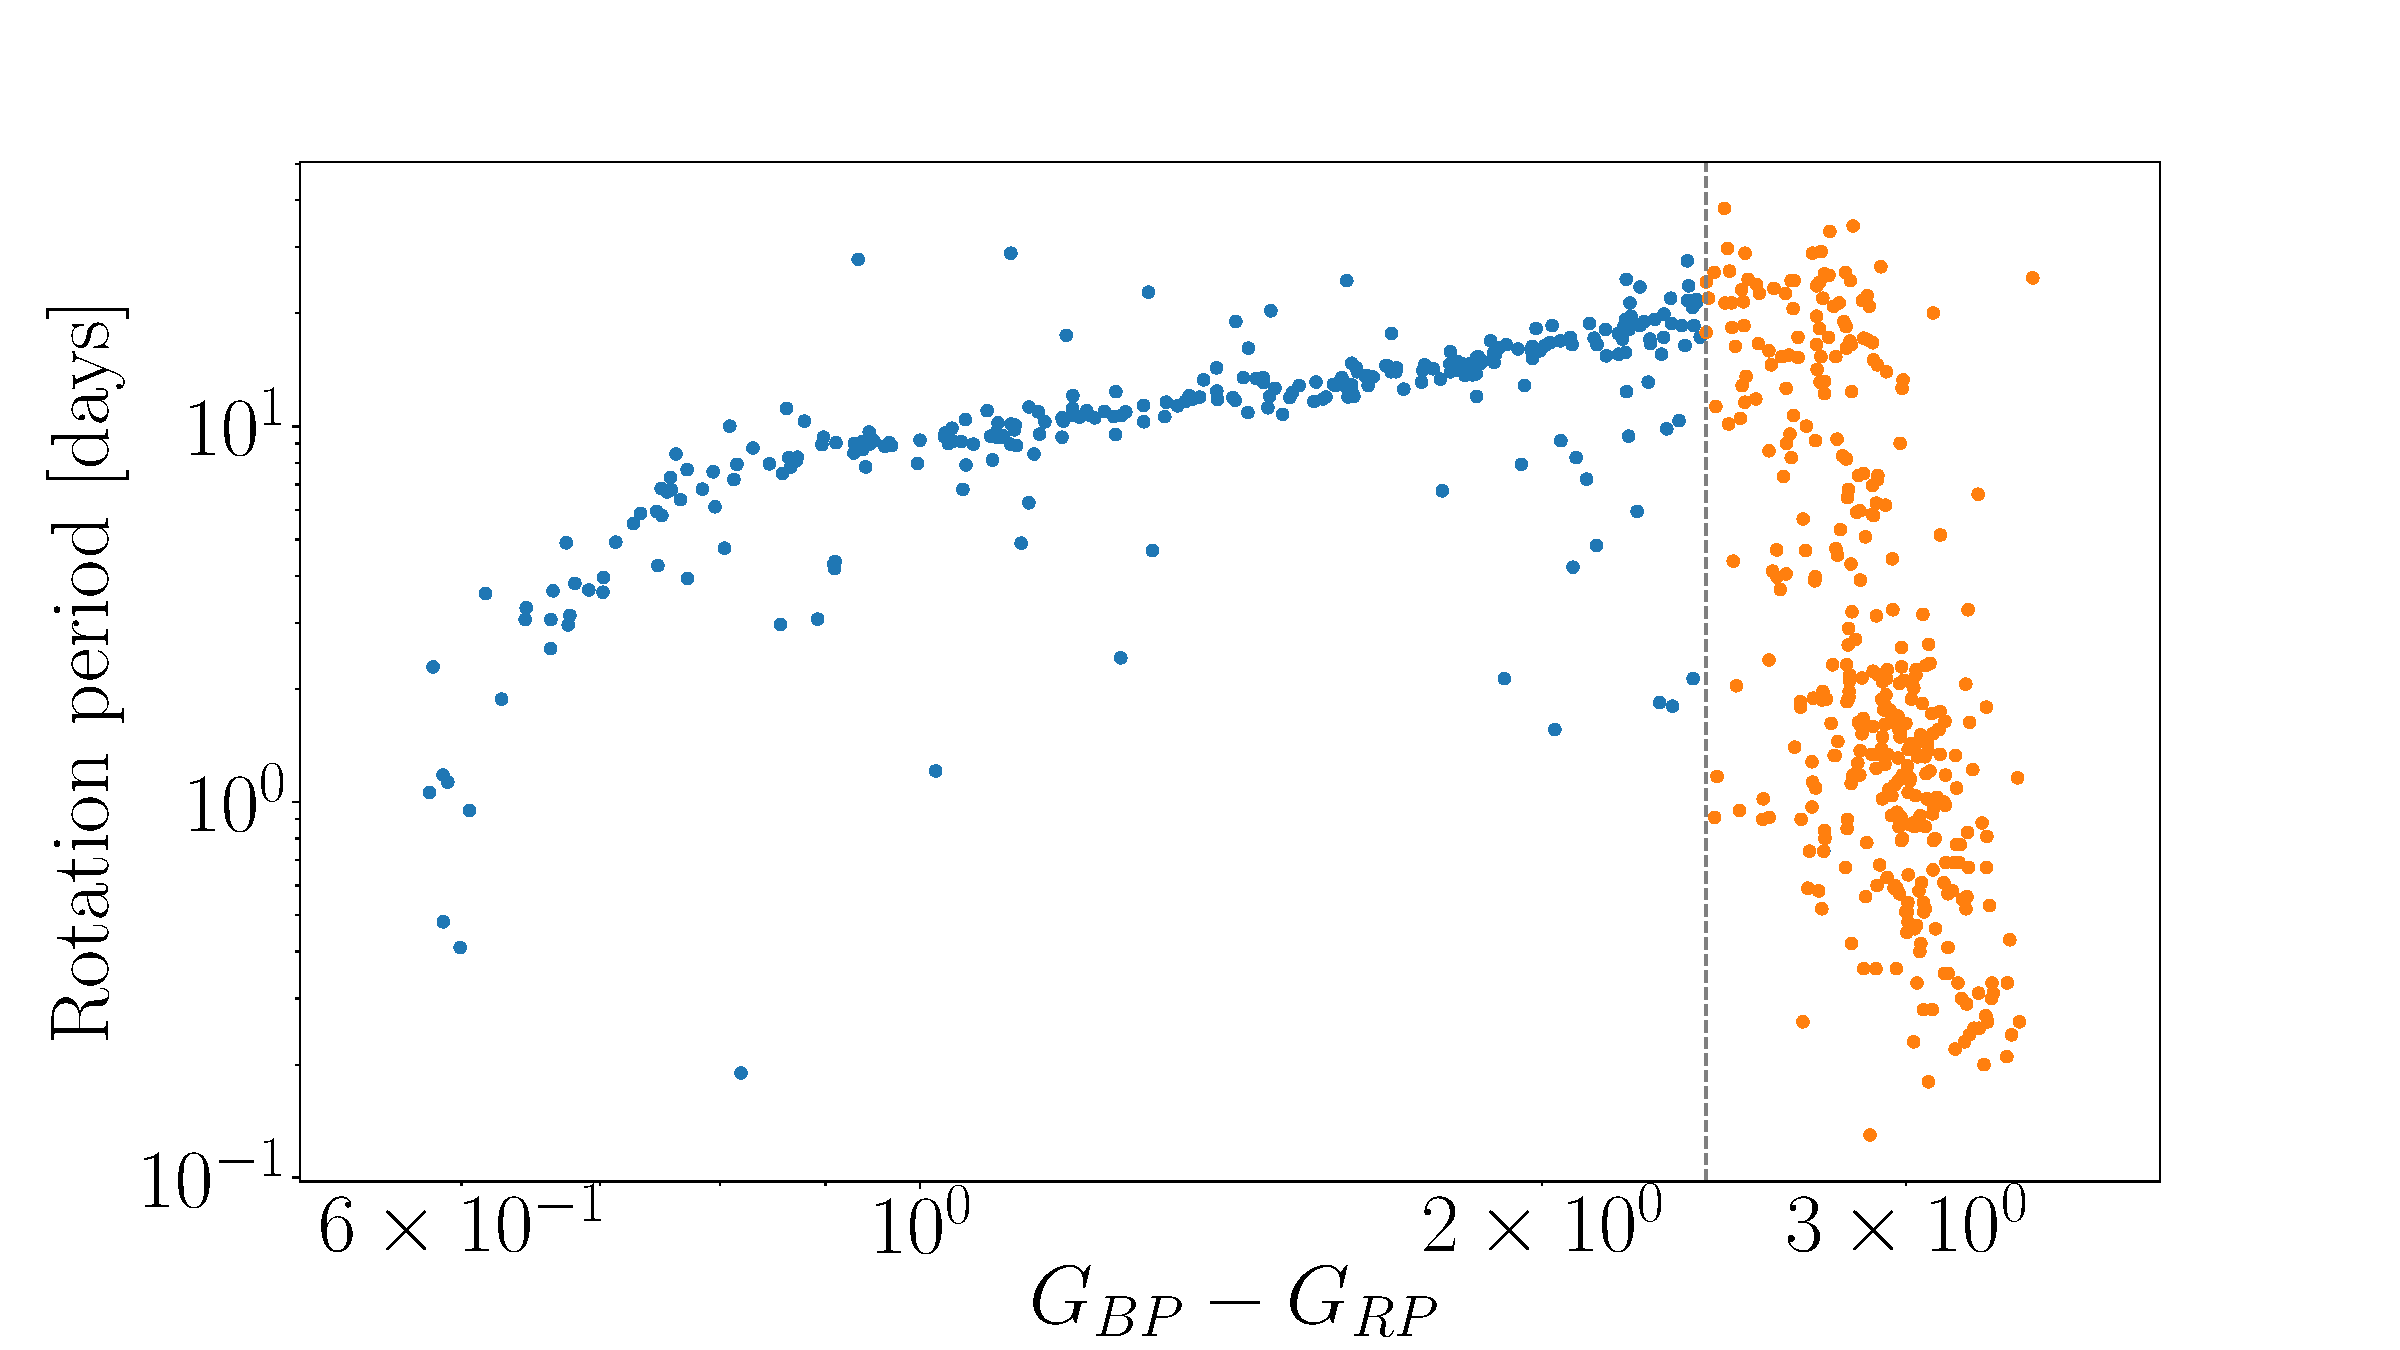
\includegraphics[width=1.1\textwidth]{praesepe}
\label{fig:praesepe}
\end{figure}
In order to fit a relation to Praesepe, we removed rotational outliers bluer
than \gcolor\ = 2.7 via sigma-clipping and fit a 5th-order polynomial to the
remaining FGK and early M stars.
\racomment{We found that a 5th order polynomial provided a substantially
better fit than lower-order polynomials, which were not able to capture the
sharp `elbow’ in the rotation period-color relation. Additional orders
provided either a worse
fit, tending towards extreme values at the boundaries, or diminishing returns
in goodness-of-fit.}
We also fit a straight line to the late M dwarfs (\gcolor\ $>$ 2.7), to
capture the mass-dependent initial rotation periods of low mass stars
\citep{somers2017}.
We fit a separable straight line function to the period-age relation using
the ages of Praesepe and the Sun\footnote{The fitting process was
performed in a Jupyter notebook available at
\url{https://github.com/RuthAngus/stardate/blob/master/paper/code/Fitting_Praesepe.ipynb}.}.
This new Praesepe-calibrated gyrochronology relation is,
\begin{equation}
    \log_{10}(P_\mathrm{rot}) =
    c_A\log_{10}(t) +
    \sum_{n=0}^4 c_n[\log_{10}(G_{BP}-G_{RP})]^n
\label{eqn:fgk_gyro}
\end{equation}
for stars with \gcolor\ $<$ 2.7 and
\begin{equation}
    \log_{10}(P_\mathrm{rot}) =
    c_A\log_{10}(t) +
    \sum_{m=0}^1 b_m[\log_{10}(G_{BP}-G_{RP})]^m
\label{eqn:m_gyro}
\end{equation}
for stars with \gcolor\ $>$ 2.7, where $P_{\mathrm{rot}}$ is rotation period
in days and $t$ is age in years.
Best-fit coefficient values are shown in table \ref{tab:coefficients}.
\begin{table}[h!]
  \begin{center}
      \caption{Coefficient values for equations \ref{eqn:fgk_gyro} and
      \ref{eqn:m_gyro}.}
    \label{tab:coefficients}
    \begin{tabular}{l|c} % <-- Alignments: 1st column left and 2nd middle, with vertical lines in between
      Coefficient & Value  \\
      \hline
      $c_A$ & 0.65 $\pm$ 0.05 \\
      $c_0$ & -4.7 $\pm$ 0.5 \\
      $c_1$ & 0.72 $\pm$ 0.05 \\
      $c_2$ & -4.9 $\pm$ 0.2 \\
      $c_3$ & 29 $\pm$ 2 \\
      $c_4$ & -38 $\pm$ 4 \\
      $b_0$ & 0.9 $\pm$ 0.5 \\
      $b_1$ & -13.6 $\pm$ 0.1 \\
    \end{tabular}
  \end{center}
\end{table}

We calibrated this new relation using Praesepe and the Sun alone, without
including other clusters, because different open clusters have slightly
different period-color relationships \citep{agueros2018, agueros2018b,
curtis2018, curtis2019} and, given that we used an age-color separable
relation, adding in extra clusters was unlikely to improve the calibration.
We did not include asteroseismic stars because most are slightly evolved and
would require a gyrochronology relation that depends on $\log g$.
This new relation, fit to Praesepe and the Sun, does not perfectly predict the
rotation periods of stars at all colors and ages, but it provides several
improvements over previous empirical gyrochronology relations.
Firstly, it uses new \ktwo\ rotation period measurements to model the
period-color relation of Praesepe in detail, secondly, it includes a model for
the rotational behavior of M dwarfs, and thirdly, it is calibrated to \Gaia\
\gcolor\ color: a directly observable quantity and the most widely available
photometric color index.

Equation \ref{eqn:fgk_gyro}, describing the rotational evolution of FGK and
early M stars, is most closely analogous to previously calibrated empirical
gyrochronology relations \citep[\eg][]{barnes2003, barnes2007, mamajek2008,
barnes2010, angus2015}.
It describes stars with Sun-like magnetic dynamos that follow a
`Skumanich-like' magnetic braking law, \ie\ their rotation period increases
with the square root of their age.
It does not describe stars hotter than around 6250 K which have a thin
convective layers and a weak magnetic dynamo, nor does it describe fully
convective stars which take a long time to converge onto the
\citet{skumanich1972} braking law \citep{krishnamurthi1997}.
In addition, stars with Rossby numbers larger than around 2 do not show
Skumanich-like magnetic braking \citep{vansaders2016, vansaders2018}, so
equation \ref{eqn:fgk_gyro} does not describe these stars.
It also does not describe the rotation periods of subgiants or giants, whose
rotation periods are influenced by their expanding radii, changing winds, and
core-to-surface differential rotation \citep[\eg][]{vansaders2013, tayar2018}.
Finally, this relation does not describe the rotation periods of dynamically
or magnetically interacting binaries which often rotate more rapidly than
isolated stars at the same age and color \citep{douglas2016}.
In order to include non-Skumanich type stars in our combined gyrochronal and
isochronal model, we designed a composite gyrochronology relation which
describes a mean and variance model for the rotation period distributions
across the HRD.
Rotation periods are modeled differently for stars of different photometric
color, EEP, Rossby number, age and metallicity.
The rotation period model for each of these groups is described below.
\begin{itemize}
    \item{The rotation periods of late F, GK, and early M dwarfs
        (0.56 $<$ \gcolor\ $<$ 2.7), with Rossby numbers less than 2, are
        modeled as a log-normal distribution, with mean given by equation
        \ref{eqn:fgk_gyro}, and variance given by the squared inverse of their
        observational uncertainties.}
    \item{The rotation periods of fully convective stars (\gcolor\ $>$ 2.7)
        are modeled with a log-normal distribution with mean given by equation
        \ref{eqn:m_gyro}, and an extra standard deviation of
        0.5 dex, added to observational uncertainties.
        This distribution reflects the observed rotation periods of late M
        dwarfs in the Praesepe cluster which span a broad range at every
        color.
        Late M dwarfs with masses $\lesssim$ 0.3 M$_\odot$, temperatures
        $\lesssim$ 3500 and \gcolor $\gtrsim$ 2.7 exhibit weak magnetic
        braking until at least after the age of Praesepe ($\sim$650 million
        years).
    \item{The rotation periods of F-type and hotter stars, with \gcolor\ $<$
        0.56 dex, are modeled as a log-normal distribution with mean,
        $\log_{10}(P_\mathrm{rot})=0.56$,
        and an additional standard deviation, added to observational
        uncertainties, of 0.5 dex.
        Stars more massive than around 1.25 M$_\odot$, with a temperature
        $\gtrsim$ 6250 K and a \gcolor\ $\lesssim$ 0.56 do not spin down
        appreciably over their main-sequence lifetimes because they do not
        have the deep convective envelope needed to generate strong magnetic
        fields.
        This model for the mean and variance of hot star rotation periods is
        based on stars hotter than 6250 K in the \citet{mcquillan2014} sample,
        which have a mean $\log_{10}(P_\mathrm{rot})$ of 0.56 dex and a
        standard deviation of around 0.5 dex.}
        Both hot and cool stars retain rotation periods that are similar to
        their primordial distribution \citep[see \eg][]{matt2012,
        somers2017}.}
    \item{The rotation periods of stars with large Rossby numbers are
        modeled as follows.
        The age at which a star's Rossby number would exceed 2 is calculated
        by inverting equation \ref{eqn:fgk_gyro}.
        If a star's age is greater than this, its mean rotation period is
        given by $P_\mathrm{max} = 2/\tau$, where $\tau$ is the convective
        turnover timescale, calculated via stellar mass using equation 11 from
        \citet{wright2011}.}
    \item{The rotation periods of subgiants are described with a log-normal
        distribution with mean given by equation \ref{eqn:fgk_gyro},
        \ref{eqn:m_gyro} or 0.56, depending on its color, and an additional
        standard deviation of 5 dex.
        This is not an accurate model of subgiant rotation
        periods \citep[see, \eg][]{vansaders2013} but the highly
        inflated variance makes it a weakly constraining one.
        Isochrone fitting provides precise ages for subgiants, so by inflating
        the variance of the gyrochronology relation at large EEP, we allow a
        star's position on the HRD/CMD to dominate the age information over
        its rotation period.
        This is useful because we have not yet built an accurate rotation-age
        relation for subgiants into our model.}
    \item{We model stars younger than around 250 Myrs with a log-normal
        distribution with mean function given by equation \ref{eqn:fgk_gyro},
        \ref{eqn:m_gyro} or 0.56, depending on it whether it has
        an intermediate, red, or blue color respectively and a inflated
        standard deviation of 0.5 dex.
        Rotation periods in young open clusters show a large amount of scatter
        because they have not yet converged onto the \citet{skumanich1972}
        spin-down sequence.}
    \item{Finally, we model stars with very low and high metallicites (-0.2
        $>$ [Fe/H] $>$ 0.2) with a log-normal distribution with mean given by
        equation \ref{eqn:fgk_gyro}, \ref{eqn:m_gyro} or 0.56, depending on
        its color, and a standard deviation of 0.5 dex.
        Gyrochronology is not calibrated at these extreme metallicities due to
        a lack of suitable metal poor and rich calibration stars.
        Rather than assume the same gyrochronology model can be na\"ively
        applied to these stars, we take a more conservative approach and model
        them with a broad Gaussian distribution.}
\end{itemize}
Inflating the variance of the rotation period distribtion for stars with
non-Skumanich magnetic braking behavior has two purposes: 1) in the cases of
hot stars and fully convective stars, it allows the broad distributions of
rotation periods observed in clusters and the field to be matched, and 2) it
down-weights the age-information provided by rotation periods in regions of
the HRD/CMD where rotation periods are not information-rich or the
gyrochronology model is inaccurate or uncalibrated.
If the observational uncertainties on rotation periods are 5\% on average,
which corresponds to 0.05/$\ln(10)$ $\sim$ 0.02 dex, adding 0.5 amounts to
a 25$\times$ increase in standard deviation, or a $\sim$ 600$\times$ increase
in variance.
% The variance on stellar ages inferred via gyrochronology is directly
% proportional to the variance on rotation periods, so a 600$\times$ increase
% in period variance corresponds to a 600$\times$ reduction in the
% age-information provide by gyrochronology, a 600$\times$ increase in
% gyrochronal age variance and a 25$\times$ increase in gyrochronal standard
% deviation.
So, practically speaking, when the standard deviation is inflated to 0.5 dex
or more, ages are almost entirely inferred via isochrone fitting.


We used the following composite gyrochronology model to infer ages from
rotation periods,
\begin{equation}
    \log_{10}(P_\mathrm{rot}) \sim \begin{cases}
        \mathcal{N}\left[(\ref{eqn:fgk_gyro}), (\sigma+\sigma_P)^2\right], & Ro < 2,
        0.56 < G_{BP} - G_{RP} < 2.7 \\
        \mathcal{N}[(\ref{eqn:m_gyro}), (\sigma+\sigma_P)^2], & Ro < 2,
        G_{BP} - G_{RP} > 2.7 \\
        \mathcal{N}[\log_{10}(P_\mathrm{max}), (\sigma+\sigma_P)^2],& Ro \geq 2 \\
        \mathcal{N}[0.56, (\sigma+\sigma_P)^2],& G_{BP} - G_{RP} < 0.56,
    \end{cases}
\label{eqn:gyro}
\end{equation}
where $\sigma$ is the relative period uncertainty, divided by $\ln(10)$, on
individual rotation period measurements and $\sigma_P$ is an additional
scatter that is a function of EEP, age, metallicity and color.
It takes a maximal value of 0.5 for hot stars and fully convective stars, 5
for subgiants and giants, and a minimal value of zero for late F, GK and early
M dwarfs.
The variance model is shown in figure \ref{fig:variance}.
Sigmoid functions were used to provide smooth transitions between regions of
low and high variance.
Sharp changes in variance would produce sharp changes in likelihood, which
would cause the posterior distributions over stellar parameters to be more
difficult to sample.
The sigmoid functions shown in figure \ref{fig:variance} reach half their
maximum values at \gcolor\ = 0.56 and 2.5 for hot and cool stars respectively,
EEP = 454 for subgiants, age = 250 Myrs for young stars, $[$M/H$]$ = -0.2 for
metal poor stars and 0.2 for metal rich stars.
The logistic growth rate, or steepness, of the sigmoid functions is 100
dex$^{-1}$ for both color transitions, .2 EEP$^{-1}$ for the EEP transition,
20 dex$^{-1}$ for the age transition and 5 dex$^{-1}$ for the both metallicity
transitions.
The additional standard deviation is additive, so if a star is \eg\ hot,
evolved and metal poor, the additional standard deviation of its rotation
period rises to 6.

\begin{figure}
  \caption{
    The additional rotation period scatter, $\sigma_P$, added to the
    observational period uncertainties in the model (see equation
    \ref{eqn:gyro}).
    The standard deviation was increased for early F and hotter
    stars (\gcolor $<$ 0.56), late M dwarfs (\gcolor\ $>$ 2.7) and evolved
    stars (EEP $\gtrsim$ 420) in order to down-weight the age-information
    supplied
    by rotation periods and reproduce observed rotation period distributions.
    We also increased the variance for stars younger than around 250 Myrs,
    because the rotation periods of these stars typically have not yet
    converged onto a tight gyrochronology sequence, and for very high and low
    metallicity stars (-0.2 $\gtrsim$ [Fe/H] $\gtrsim$ 0.2) because the
    gyrochronology relations have not been calibrated at these extreme values.
    Down-weighting the gyrochronal likelihood by the inverse variance
    ($1/\sigma^2$) allowed the ages of these stars to be mostly inferred
    via isochrone fitting.
    Sigmoid functions were used to provide smooth transitions between regions
    of low and high variance.
}
  \centering
    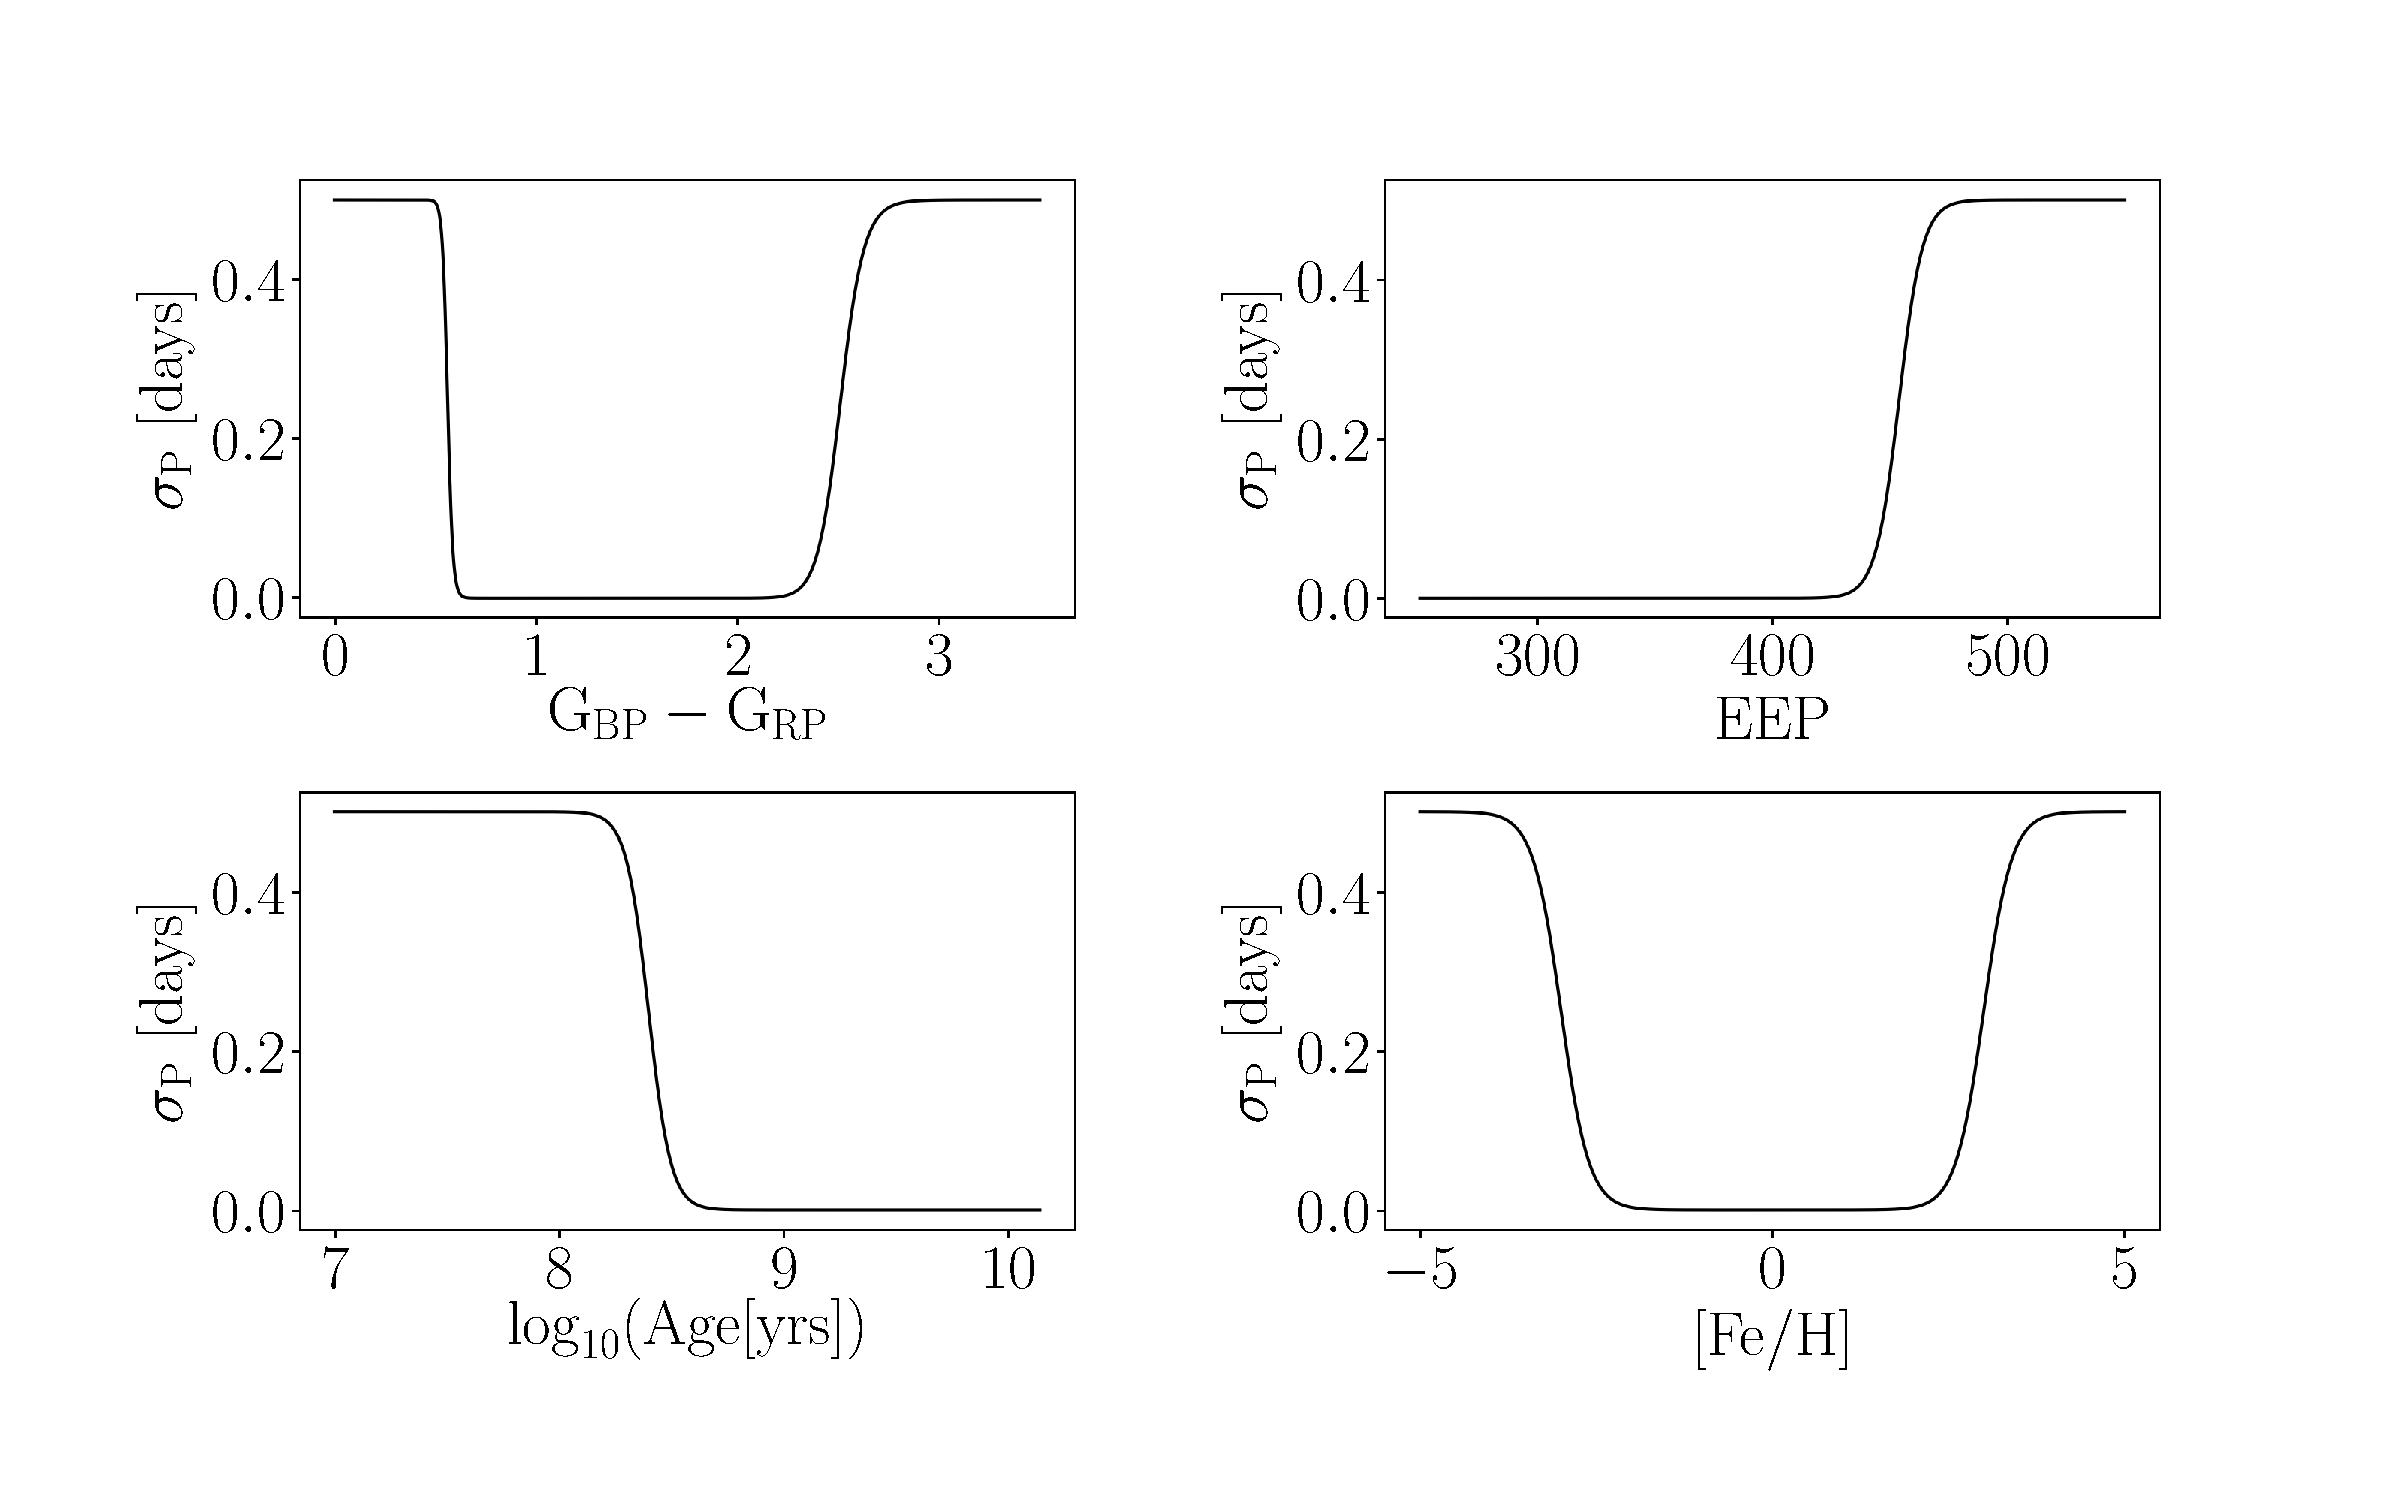
\includegraphics[width=1.\textwidth]{variance}
\label{fig:variance}
\end{figure}

\subsection{Simultaneously fitting gyrochronology and isochrones}
The previous part of this section describes the model for the mean and
variance of rotation periods as a function of their ages (and colors, EEPs,
masses and metallicities).
In what follows, we describe how this model was combined with a stellar
evolution model to infer stellar ages (and other parameters) via
gyrochronology and isochrone fitting simultaneously.
Our goal was to infer the age of a star from its observable properties by
estimating the posterior probability density function (PDF) over age,
\begin{equation} \label{eqn:eqn1}
    % p(t|{\bf m_x}, T_{\mathrm{eff}}, \log(g), \hat{F},
    p(t|{\bf m_x}, P_{\mathrm{rot}}, \bar{\pi}),
\end{equation}
where $t$ is age, ${\bf m_x}$ is a vector of
apparent magnitudes in various bandpasses,
\prot\ is the rotation period and \pmega\ is parallax.
Spectroscopic properties (\teff, \logg\ and $\mathrm{[Fe/H]}$) and/or
asteroseismic parameters (\dnu\ and \numax) may also be available for a star,
in which case they would appear to the right of the `$|$' in the above
equation since they are observables.
In order to calculate a posterior PDF over age, other stellar parameters must
be marginalized over.
These parameters are distance ($D$), V-band extinction ($A_V$), the
inferred metallicity, $[M/H]$\footnote{The inferred metallicity, [M/H] is a
model parameter which is different to the {\it observed} metallicity, [Fe/H]
which would appear on the right side of the $`|'$ in equation \ref{eqn:eqn1}.},
and equivalent evolutionary phase (abbreviated to EEP or
$E$).
EEP is a dimensionless number ranging from around 200 for M dwarfs up
to around 1600 for giants and is 355 for the Sun \citep[see][]{dotter2016,
choi2016}.
Stars are defined as subgiants when their EEP exceeds 454.
Mass is uniquely defined by EEP, age and metallicity.
The marginalization involves integrating over these extra parameters,
\begin{eqnarray} \label{eqn:bayes}
    % & p(A|{\bf m_x}, T_{\mathrm{eff}}, \log(g), \hat{F},
    & p(t|{\bf m_x},
    P_{\mathrm{rot}}, \bar{\pi})
\\ \nonumber
    % & \propto \int p({\bf m_x}, T_{\mathrm{eff}}, \log(g), \hat{F},
    & \propto \int p({\bf m_x},
    P_\mathrm{rot}, \bar{\pi}|
    t, E, [M/H], D, A_V)~p(t)\, p(E)\, p([M/H])\, p(D)\, p(A_V)\, \mathrm{d}E\,
    \mathrm{d}[M/H]\, \mathrm{d}D\, \mathrm{d}A_V.
\end{eqnarray}
This equation is a form of Bayes' rule,
\begin{equation} \label{eqn:eqn2}
\mathrm{Posterior} \propto \mathrm{Likelihood} \times \mathrm{Prior},
\end{equation}
where the likelihood of the data given the model is,
\begin{equation} \label{eqn:full_likelihood}
    % p({\bf m_x}, T_{\mathrm{eff}}, \log(g), \hat{F}, \bar{\pi},
    p({\bf m_x}, \bar{\pi}, P_{\mathrm{rot}}|t, E, D, A_V, [M/H]),
\end{equation}
and the prior PDF over parameters is,
\begin{equation} \label{eqn:prior}
    p(t)\, p(E)\, p(D)\, p(A_V)\, p([M/H]).
\end{equation}
The priors we used are described in the appendix.

We assumed that the process of magnetic braking is independent of hydrogen
burning in the core, outside of the dependencies that are captured in the
model.
This assumption allowed us to multiply two separate likelihood
functions together: one computed using an isochronal model and one computed
using a gyrochronal model.
We assumed that the probability of observing the measured observables given
the model parameters was a Gaussian and that the observables were identically
and independently distributed.
The isochronal likelihood function was,
\begin{eqnarray} \label{eqn:isochrones_only_likelihood}
    % & \mathcal{L_{\mathrm{iso}}} = p({\bf m_x}, T_{\mathrm{eff}}, \log(g),
    & \mathcal{L_{\mathrm{iso}}} = p({\bf m_x},
    \bar{\pi}|t, E, [M/H], D,
    A_V) \\ \nonumber
    & = \frac{1}{\sqrt{(2\pi)^n \det(\Sigma)}}
    \exp\left( -\frac{1}{2} ({\bf O_I} - {\bf I})^T \Sigma ^{-1}
    ({\bf O_I} - {\bf I})\right),
\end{eqnarray}
where ${\bf O_I}$ is the vector of n observables: \pmega, ${\bf m_x}$ plus
spectroscopic and/or asteroseismic observables if available, and $\Sigma$ is
the covariance matrix of that set of observables.
${\bf I}$ is the vector of {\it model} observables that correspond to a set of
parameters: $t$, $E$, $[M/H]$, $D$ and $A_V$, calculated using an isochrone model.
We assumed there is no covariance between these observables and so this
covariance matrix consists of individual parameter variances along the
diagonal with zeros everywhere else.
The gyrochronal likelihood function was,
\begin{eqnarray} \label{eqn:gyro_likelihood}
    & \mathcal{L_{\mathrm{gyro}}} = p(P_\mathrm{rot} |t, E, [M/H], D, A_V) \\ \nonumber
    & = \frac{1}{\sqrt{(2\pi) \det(\Sigma_P)}}
    \exp\left( -\frac{1}{2} ({\bf P_O} - {\bf P_P})^T \Sigma_P ^{-1}
    ({\bf P_O} - {\bf P_P})\right),
\end{eqnarray}
where ${\bf P_O}$ is a 1-D vector of observed logarithmic rotation periods,
and ${\bf P_P}$ is the vector of corresponding logarithmic rotation periods,
predicted by the model.
$\Sigma_P$ was comprised of individual rotation period measurement
uncertainties, plus an additional variance that is a function of EEP and
\gcolor\
color, added in quadrature.
This variance accounts for the stochastic nature of the rotation periods of
very hot and very cool stars and allowed us to predominantly use isochrone
fitting to measure the ages of subgiants.
The full likelihood used in our model was the product of these two likelihood
functions,
\begin{equation}
    \mathcal{L}_{\mathrm{full}} = \mathcal{L}_{\mathrm{iso}} \times
    \mathcal{L}_{\mathrm{gyro}}.
\end{equation}

The inference processes proceded as follows.
First, a set of parameters: age, EEP, metallicity, distance and extinction,
and observables for a single star were passed to the isochronal likelihood
function in equation \eqref{eqn:isochrones_only_likelihood}.
Then, a set of observables corresponding to those parameters were generated
from the MIST model grid using {\tt isochrones.py} \citep{isochrones} and
compared to the measured observables via the isochronal likelihood,
$\mathcal{L}_{\mathrm{iso}}$ (also computed using {\tt isochrones.py}).
The parameters were also passed to the gyrochronology model (equation
\ref{eqn:gyro}) where $t$, $E$,
$[M/H]$, $D$ and $A_V$ were used to calculate \gcolor\ color and mass from the
MIST model grid and, in turn, rotation period via the gyrochronology model.
EEP and \gcolor\ were also used to calculate the additional rotation period
variance, added to the individual period uncertainties.
This model rotation period was compared to the measured rotation period using
gyrochronal likelhood function of equation \ref{eqn:gyro_likelihood}.
The gyrochronal log-likelihood was added to the isochronal log-likelihood to
give the full likelihood, which was then added to the log-prior to produce a
single sample from the posterior PDF.

Ages were inferred with \sd\ using Markov Chain Monte Carlo.
The joint posterior PDF over age, mass, metallicity, distance and extinction
was sampled using the affine invariant ensemble sampler, {\tt emcee}
\citep{foreman-mackey2013} with 50 walkers.
Samples were drawn from the posterior PDF until 100 {\it independent} samples
were obtained.
We actively estimated the autocorrelation length, which indicates how many
steps were taken per independent sample, after every 100 steps using the
autocorrelation tool built into {\tt emcee}.
The MCMC concluded when {\it either} 100 times the autocorrelation length was
reached and the change in autocorrelation length over 100 samples was less
than 0.01, {\it or} the maximum of 500,000 samples was obtained.
This method is trivially parallelizable, since the inference process for each
star can be performed on a separate core.
The age of a single star can be inferred in around 1 hour on a laptop
computer.

\section{Results}
\label{section:results}

In order to demonstrate the performance of our method, we conducted three sets
of tests.
In the first we simulated observables from a set of stellar parameters for a
few hundred stars using the MIST stellar evolution models and the
gyrochronology model of equation \ref{eqn:gyro}.
The ages predicted with our model were compared to the true parameters used to
generate the data.
In the second we tested our model by measuring the ages of individual stars in
the NGC 6819 open cluster, and in the third we tested our model on \kepler\
asteroseismic stars.

\subsection{Test 1: simulated stars}
For the first test we drew masses, ages, bulk metallicities, distances and
extinctions at random for 1000 stars from the following uniform distributions:
\begin{eqnarray}
& \mathrm{EEP} \sim U(198, 480) \\
% & M \sim U(0.5, 1.5)~[M_\odot] \\
& t \sim U(0.5, 14)\mathrm{~[Gyr]} \\
& [Fe/H] \sim U(-0.2, 0.2) \\
& D \sim U(10, 1000)~\mathrm{[pc]} \\
& A_V \sim U(0, 0.1).
\end{eqnarray}
\teff, \logg, \fhat, parallax, and apparent magnitudes $B$, $V$, $J$, $H$, $K$,
\gaia\ $G$, $G_{BP}$ and $G_{RP}$ were generated from these
stellar parameters using the MIST stellar evolution models.
We added a small amount of noise to the `observed' stellar properties in order
to reflect optimistic observational uncertainties for isochrone-dating.
We added Gaussian noise with a standard deviation of 25 K to \teff, 0.01 dex
to \feh\ and \logg, and 10 mmags to $B$, $V$, $J$, $H$, and $K$ magnitudes.
These are just one choice of uncertainties that we could have adopted and are
extremely optimistic.
The uncertainties on predicted ages {\it will} depend strongly on all
observational uncertainties, however, since this analysis is designed to show
the relative improvement in stellar age precision when {\it rotation periods}
are included, we chose to use best-case spectroscopic parameters.
The noise added to Gaia $G$-band photometry ranged from
0.3 mmag for stars brighter than 13th magnitude, to 10 mmag for stars
around 20th magnitude \citep{evans2017, brown2018}.
Noise added to \gaia\ $G_{BP}$ and $G_{RP}$ bands ranged from 2 mmag for stars
brighter than 13th magnitude to 200 mmag for stars fainter than 17th.
Unphysical combinations of stellar parameters were discarded, resulting in a
final sample size of 841 simulated stars.
Figure \ref{fig:CMD_age} shows the position of these stars on an HRD
(with \logg\ on the y-axis instead of luminosity to improve the visibility of
the MS), colored by their age.
Rotation periods for these stars were generated using the gyrochronology
relation described in equation \ref{eqn:gyro}.
We added 5\% Gaussian noise to all stellar rotation periods to represent
realistic measurement uncertainties of 5\%.
The median uncertainty on rotation periods calculated from \kepler\ light
curves, provided in the \citet{mcquillan2014} catalog is 1\%.
However, the \citet{aigrain2015} injection and recovery study showed that true
rotation period uncertainties are often slightly larger than this, and noise
distribution of rotation periods can be highly non-Gaussian
\citep[\eg][]{aigrain2015, angus2018}.
\begin{figure}
  \caption{
      The simulated star sample plotted on an HRD, colored by age
    (top panel) and rotation period (bottom panel).
    HRD positions were calculated using MIST isochrones via the {\tt
    isochrones.py} {\it Python} package and rotation periods were generated
    using equation \ref{eqn:gyro}.
    This figure was generated in a Jupyter notebook available at
    \url{https://github.com/RuthAngus/stardate/blob/master/paper/code/Simulate_data.ipynb}
}
  \centering
    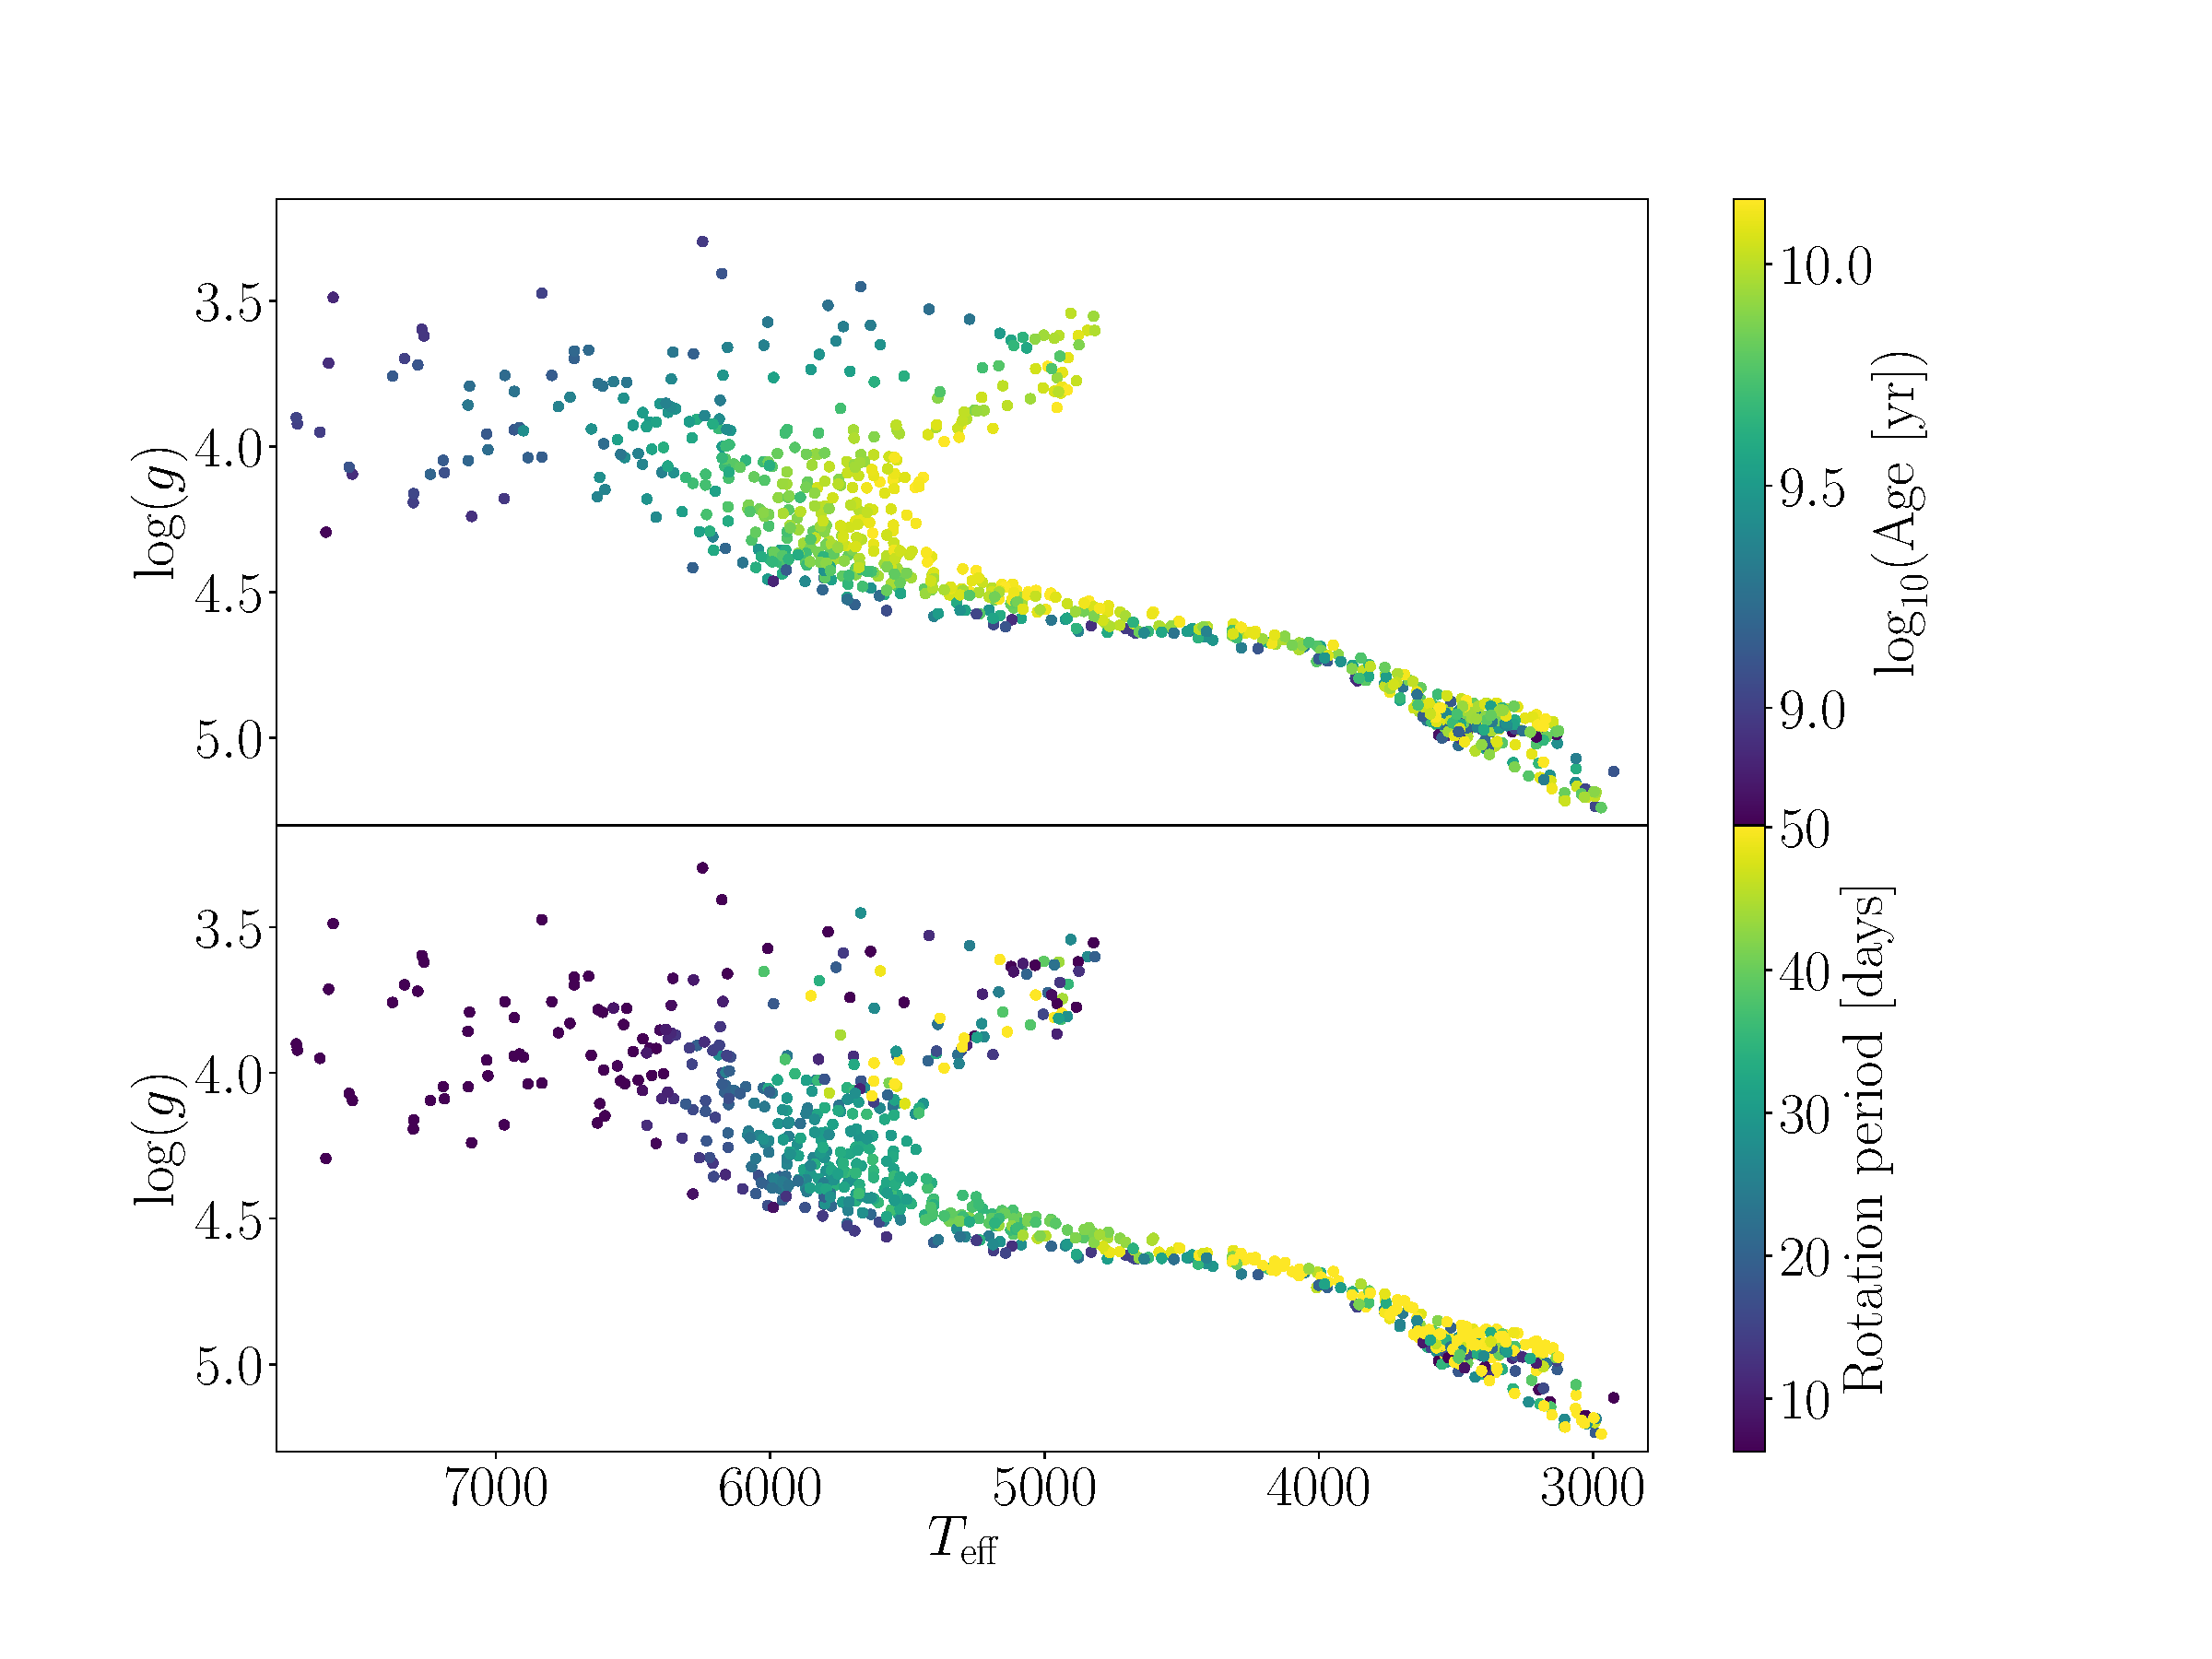
\includegraphics[width=1\textwidth]{simulated_CMD}
\label{fig:CMD_age}
\end{figure}
Figure \ref{fig:rotation_model} shows the rotation periods of 841
stars generated from the gyrochronology model.
\begin{figure}
  \caption{
Data simulated from the rotation period model.
    Late F, GK and early M dwarfs (stars with 0.56 $<$ \gcolor\ $<$ 2.7 follow
    the Praesepe-calibrated gyrochronology relation (dashed gray lines), with
    the exception of old, slowly
    rotating stars with large Rossby numbers whose rotation periods are fixed
    at 2$\times$ their convective overturn time.
    The rotation periods of early F (\gcolor $<$ 0.56), late M dwarfs (\gcolor
    $<$ 2.7) and subgiants (EEP $\gtrsim$ 420) were generated
    from a log-normal distribution with standard deviation given by equation
    \ref{eqn:gyro}.
% The top panel shows the rotation periods vs. B-V colors of simulated stars,
The top panel shows the rotation periods vs. \gcolor\ colors of simulated stars,
    colored by their age and the bottom panel shows the same stars colored
    by their equivalent evolutionary phase (EEP).
    % 9, 11, and 13 (rotation periods rise with age).
    The gray lines describe the mean gyrochronology model at ages 1,
    3, 5, 7, 9, 11, and 13 (rotation periods rise with age).
    This figure was generated in a Jupyter Notebook, available at
    \url{https://github.com/RuthAngus/stardate/blob/master/paper/code/Simulate_data.ipynb}
}
  \centering
    \includegraphics[width=1.\textwidth]{rotation_model_praesepe}
\label{fig:rotation_model}
\end{figure}

We took two approaches to inferring the ages of these simulated stars:
firstly using isochrone fitting {\it only}, and secondly using isochrone
fitting {\it combined with} a gyrochronology model (\sd).
Since the posterior PDFs of stars are often multimodal, we found that the
choice of initial positions of the {\tt emcee} walkers influenced the final
outcome because walkers occasionally got stuck in local minima.
We found that the following set of initial parameters worked well, though not
perfectly: EEP = 330, $t = 9.56$ Gyr, $[M/H] = -0.05$, $D = 269$ pc and $A_V =
0.0$\footnote{These are the default initial parameters provided in \sd.}.
Figure \ref{fig:simulation_results} shows the results of combining
gyrochronology with isochrone fitting for the simulated sample.
The stars' true ages are plotted against their predicted ages, with ages
inferred with gyrochronology and isochrone fitting
in color, and ages inferred using isochrone fitting only plotted in light
grey.
The different panels show the results for different types of stars: FGK
dwarfs that are still undergoing magnetic braking, FGK dwarfs that have ceased
magnetic braking (their Rossby number is around 2), M dwarfs, and evolved
stars.
The selection criteria for these groups are in the panel headings.
The FGK dwarfs with low Rossby numbers showed the largest improvement: the
median age precision for this group (defined as the standard deviation of the
posterior as a percentage of the median age) was 8\% when using a combination
of isochrones and gyrochronology, and 22\% using isochrone fitting alone.
This equates to an almost 3$\times$ improvement in age precision.
The age RMS of this group was 0.8 Gyr using isochrones and gyrochronology, and
2 Gyr using isochrones only.
Despite the fact that stars with Rossby numbers of 2 have stopped spinning
down and their rotation periods no longer evolve with age, the ages of these
stars can still be relatively precisely constrained with isochrone fitting.
The median age precision for stars with large Rossby numbers was 11\% with
gyrochronology and isochrone fitting, and 13\% with isochrone fitting only.
% This is because their rotation periods are still directly related to their
% age, but also {\it indirectly} related to their age via EEP and metallicity,
% as shown in equation \ref{eqn:gyro}.
% When including rotation periods to infer the ages of stars with large Rossby
% numbers, age precision improves from 21\% to 11\% and the age RMS improves
% from 2.5 to 0.9 Gyr.
% Age precision also increases for F dwarfs when incorporating their rotation
% periods, even though they are not directly related to their ages.
% This is because rotation period relates to color via the variance model in
% equation \ref{eqn:gyro}.
The precision of M dwarf ages did improve overall when their rotation periods
were included, but this improvement was entirely driven by the early M dwarfs.
The precision of this group improved overall from 33\% to 22\% and RMS from
5.4 Gyr to 4.6 Gyr.
The precision of ages inferred for evolved stars changed very little when
rotation periods were included in the inference process.
This is because the variance of the rotation-age relation was inflated by a
large amount in the gyrochronology model (equation \ref{eqn:gyro}), making
rotation periods almost entirely uninformative for this group.
The median age precision of subgiants from both gyrochronology and isochrone
fitting and isochrone fitting alone was 7\%.

\begin{figure}
  \caption{
The true vs. predicted ages of simulated stars.
    Ages calculated by combining gyrochronology
    and isochrone fitting with \sd\ are shown in color and ages calculated with
    isochrone fitting only are shown in gray.
The different panels show the results for stars
    with \gcolor\ $<$ 2.2 (FGK dwarfs) that are still braking magnetically
    ($Ro < 2$), stars with \gcolor\ $<$ 2.2 that have stopped braking
    magnetically ($Ro \geq 2$),
    stars with 2.2 $<$ \gcolor\ (M dwarfs), and evolved stars (EEP $>$ 420).
Gyrochronology is highly effective for FGK stars and ages inferred with both
    gyrochronology and isochrone fitting are more accurate and precise than
    ages inferred via isochrone fitting only for this group.
Neither gyrochronology nor isochrone fitting can provide precise ages for
    M dwarfs, so the ages of these stars are imprecise regardless of
    age-dating method.
    This figure was generated in a Jupyter Notebook available at
    \url{https://github.com/RuthAngus/stardate/blob/master/paper/code/Results_plots.ipynb}.
}
  \centering
    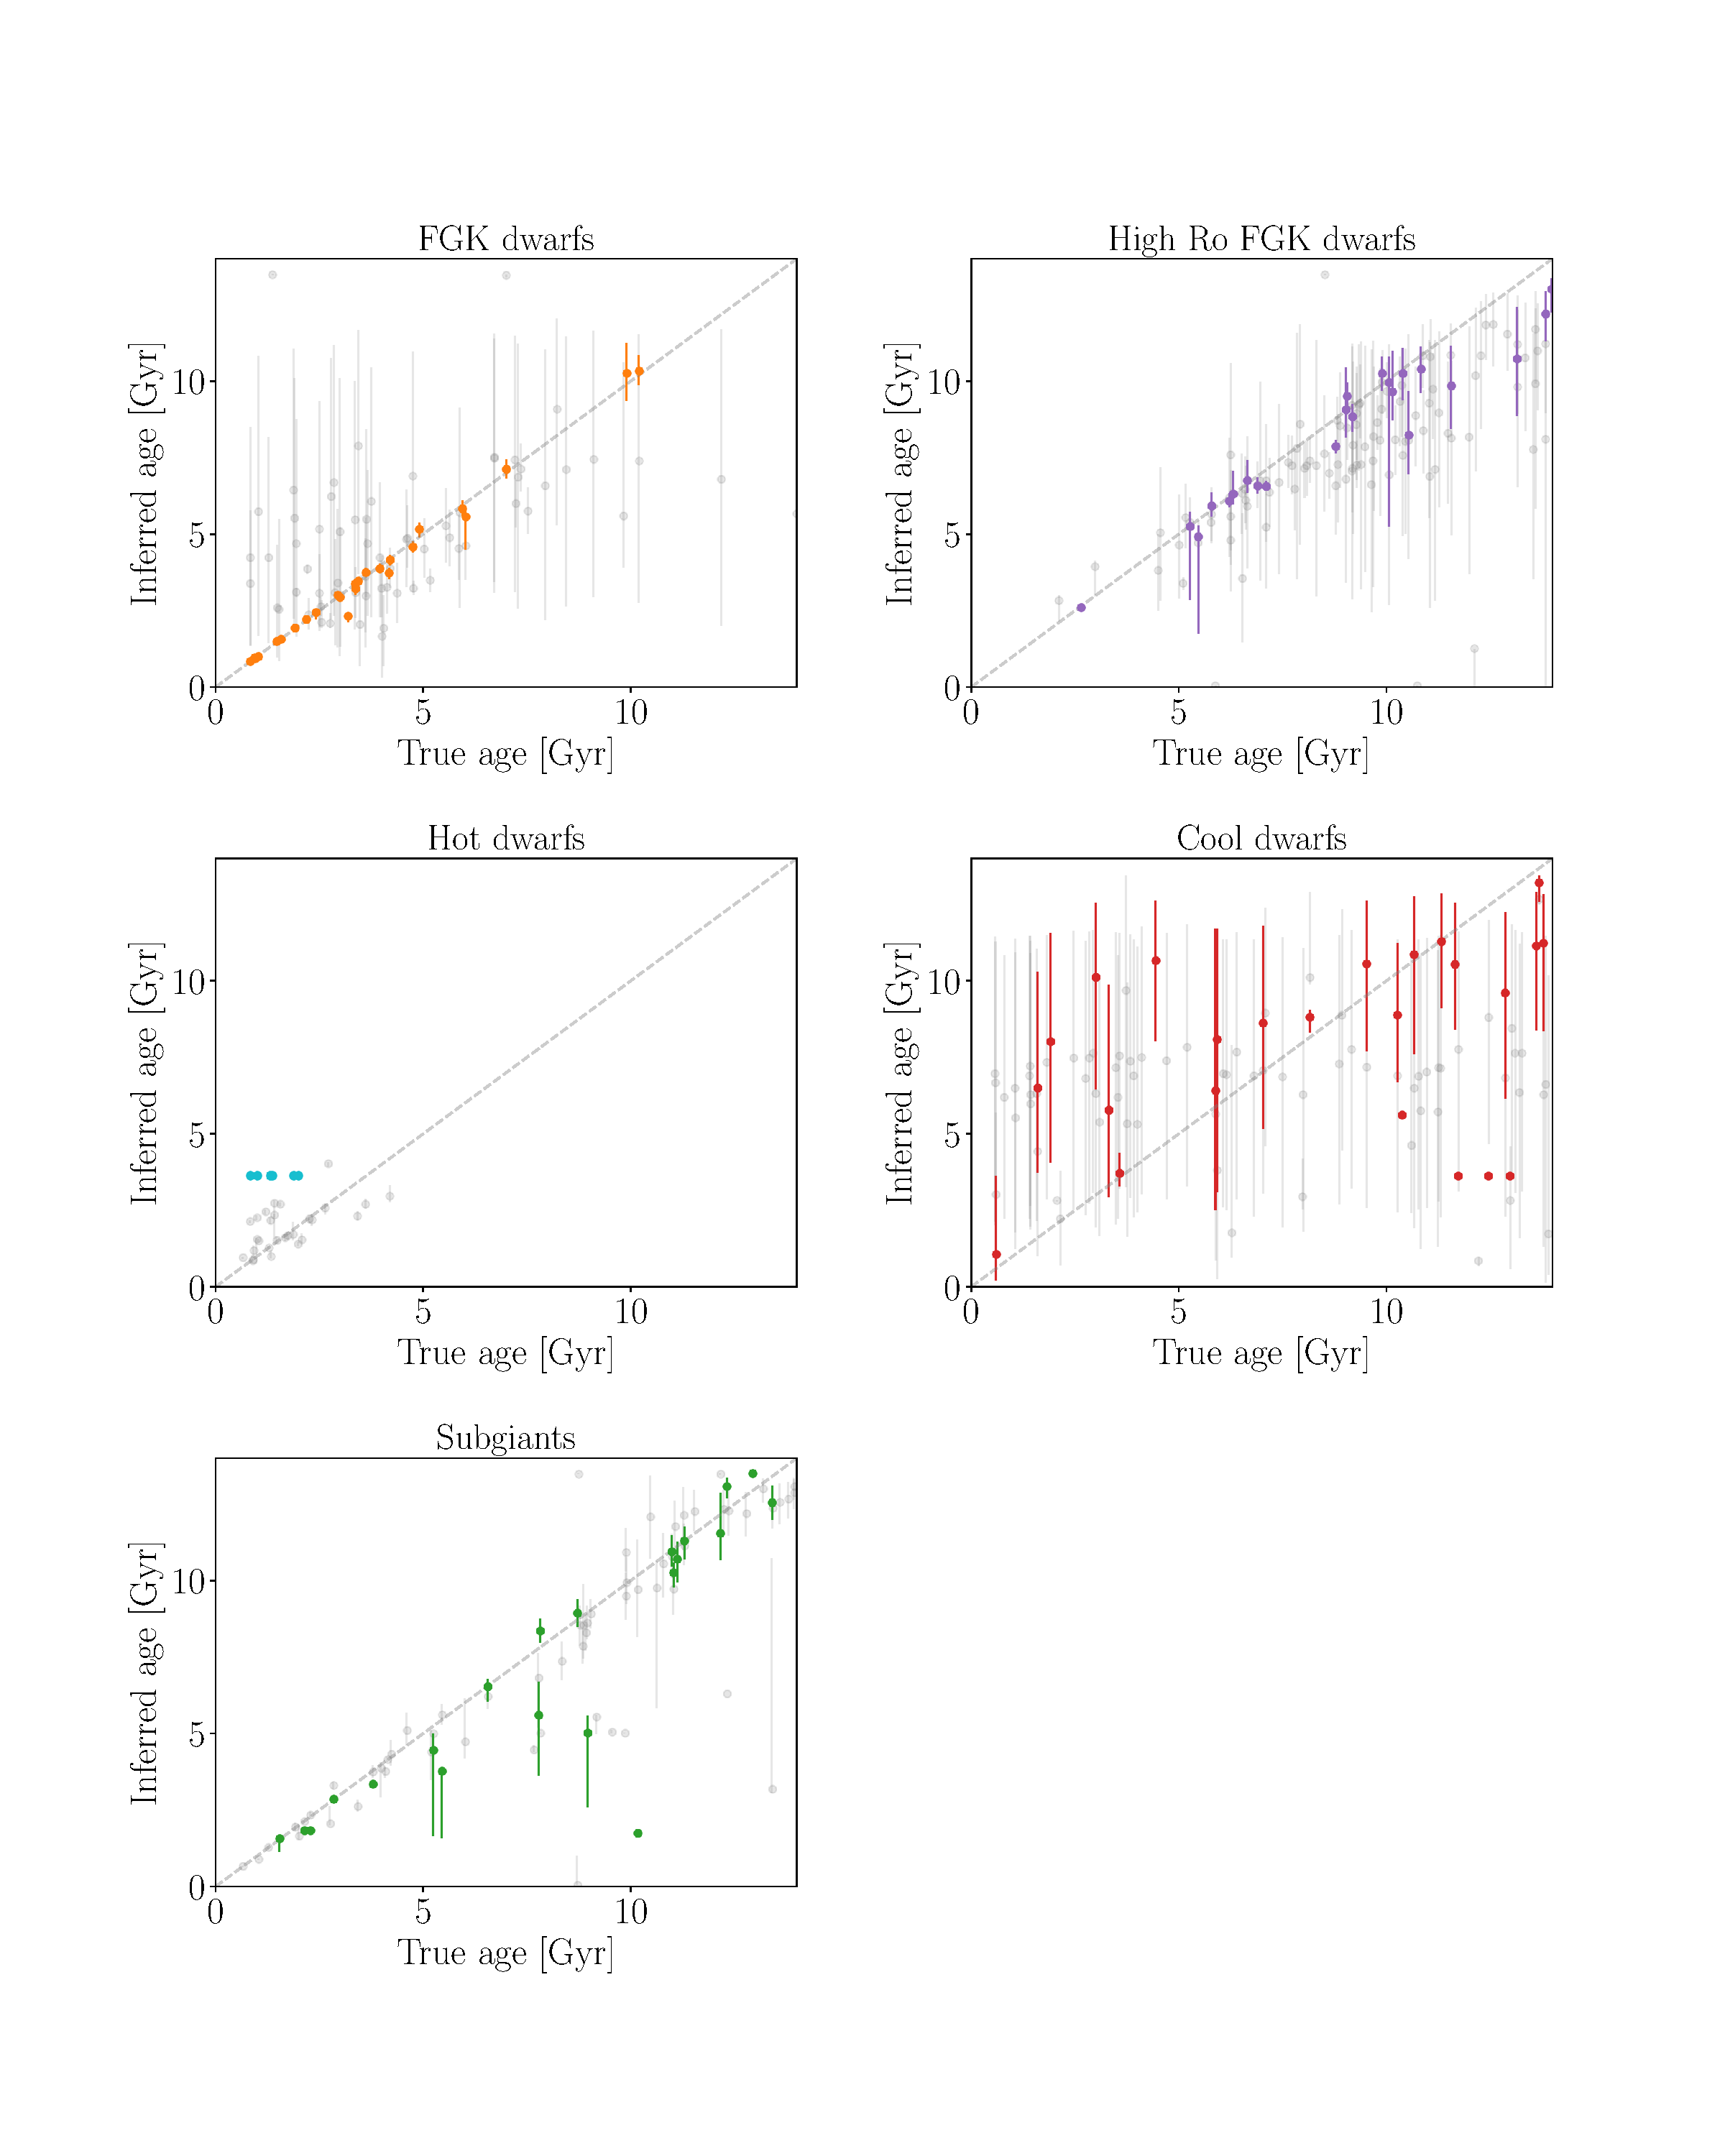
\includegraphics[width=1\textwidth]{simulation_results}
\label{fig:simulation_results}
\end{figure}

An important caveat associated with these results is that they strongly depend
on the uncertainties adopted for all observables used in the analysis: \teff,
\feh, \logg, $G$, $G_BP$, $G_RP$, $J$, $H$, $K$, $B$, $V$, and rotation
period.
Changing the uncertainties on these observables will affect the uncertainties
on inferred ages in different ways.
This demonstration is not intended to reflect the typical age uncertainties
that will result for all stars in reality, it merely exemplifies the increase
in stellar age precision that results from one specific choice of
uncertainties.
Needless to say, estimating the uncertainties on observables accurately can be
as important as accurately measuring the observables themselves.

% Figure \ref{fig:all_iso_gyr} shows the inferred vs. true ages of all simulated
% stars, colored by their \gaia\ \gcolor\ age.
% The ages of FGK stars (\gcolor\ $<$ 2.2) were more precisely recovered with
% gyrochronology and isochrone fitting than with isochrone fitting alone.
% In both cases M dwarfs ages were not precisely recovered.
% \begin{figure}
%   \caption{
%       Inferred vs. true ages for all simulated stars using isochrones plus
%       gyrochronology via the \sd\ code (left) and isochrones only (right).
%       Stellar ages are colored by \gaia\ \gcolor\ color.
%       The ages of FGK stars (\gcolor\ $<$ 2.2)
%       were more precisely recovered with \sd\ than with isochrones only.
%       In both cases M dwarfs ages were not precisely recovered.
%       Points in the lower right of the left panel are either M dwarfs or
%       evolved (EEP $>$ 400).
%       In both panels, the ages of FGK stars were slightly underestimated.
% }
%   \centering
%     \includegraphics[width=1\textwidth]{all_iso_gyro}
% \label{fig:all_iso_gyro}
% \end{figure}

% Figure \ref{fig:eep} shows the inferred equivalent evolutionary phase (EEP)
% for the simulated star sample.
% EEP is a dimensionless number that describes evolutionary stage and, combined
% with age and metallicity, determines stellar mass.
% An interesting result of inferring stellar properties with both isochrones
% {\it and} rotation periods is an increase in EEP precision, .
% The reason for this is partly that EEP and age are correlated, so shrinking
% the age posterior also shrinks the EEP posterior, and partly because rotation
% period is a function of HRD position.
% As shown in equation \ref{eqn:gyro}, rotation period does not just depend on
% color and age, but also on EEP and [Fe/H].
% \begin{figure}
%   \caption{
%     Inferred EEP for the simulated star sample with isochrones plus
%     gyrochronology (left panel) and isochrone fitting only (right panel).
%     Rotation periods provide information about position on the HRD via
% equation \ref{eqn:gyro} and therefore improve all stellar parameters, not
% just age.
%     This figure was generated in a Jupyter Notebook available at
%     \url{https://github.com/RuthAngus/stardate/blob/master/paper/code/Results_plots.ipynb}.
% }
%   \centering
%     \includegraphics[width=1\textwidth]{eep}
% \label{fig:eep}
% \end{figure}
% In general, the posterior PDFs of stellar properties, inferred using
% isochrones or stellar evolution models, are multimodal.
% The stars with under-predicted EEP in both panels of figure \ref{fig:eep} are
% slightly evolved, with EEPs $>$ 400.
% These slightly evolved stars have two high probability modes: one at their
% true EEP and age values, and another at a lower EEP and corresponding lower
% age.
% In other words, these are subgiants being mistaken for dwarfs.
% Rotation periods do not carry information for subgiants, so including the
% rotation periods in the analysis of these stars doesn't break the degeneracy,
% and this is why stars with under-predicted EEPs are present in both panels.
% Stars with over-predicted EEPs in the right-hand panel of figure \ref{fig:eep}
% are usually dwarfs being confused for subgiants.
% The rotation periods of dwarfs are informative, so when the rotation periods
% are included in the analysis for these stars, the degeneracy is broken, the
% amplitude of the secondary mode is reduced, and their EEP is correctly
% inferred.

% Figure \ref{fig:precision} shows the simulated stars on an HRD, with
% points colored by the precision of their predicted ages
% (defined as the standard deviation of the age
% posterior PDF, as a percentage of the median age).
% The top panel shows the precision of ages calculated using both gyrochronology
% and isochrone fitting via \sd\ and the bottom panel shows the precision of
% ages calculated with isochrone fitting only.
% Although these are empirical uncertainties, calculated via MCMC which only
% approximates the age posterior PDFs, they nevertheless show that combining
% gyrochronology and isochrone fitting improves age precision on the MS,
% particularly at low masses.
% \begin{figure}
%   \caption{
% Simulated stars on an HRD, colored by their relative age precision
%     using gyrochronology and isochrone fitting via \sd\ (top panel) and
%     isochrone fitting only (bottom panel).
% Combining gyrochronology with isochrone fitting significantly improves stellar
%     age precision on the MS.
% Isochrone fitting provides precise ages for hot stars and subgiants and the
%     rotation periods of these stars are relatively uninformative, so
%     gyrochronology does not significantly improve their age precision.
% The ages of late M dwarfs are highly imprecise because their ages are not well
%     determined by either their rotation periods or their position on the HRD
%     or CMD.
%     This figure was generated in a Jupyter Notebook available at
%     \url{https://github.com/RuthAngus/stardate/blob/master/paper/code/Results_plots.ipynb}.
% }
%   \centering
%     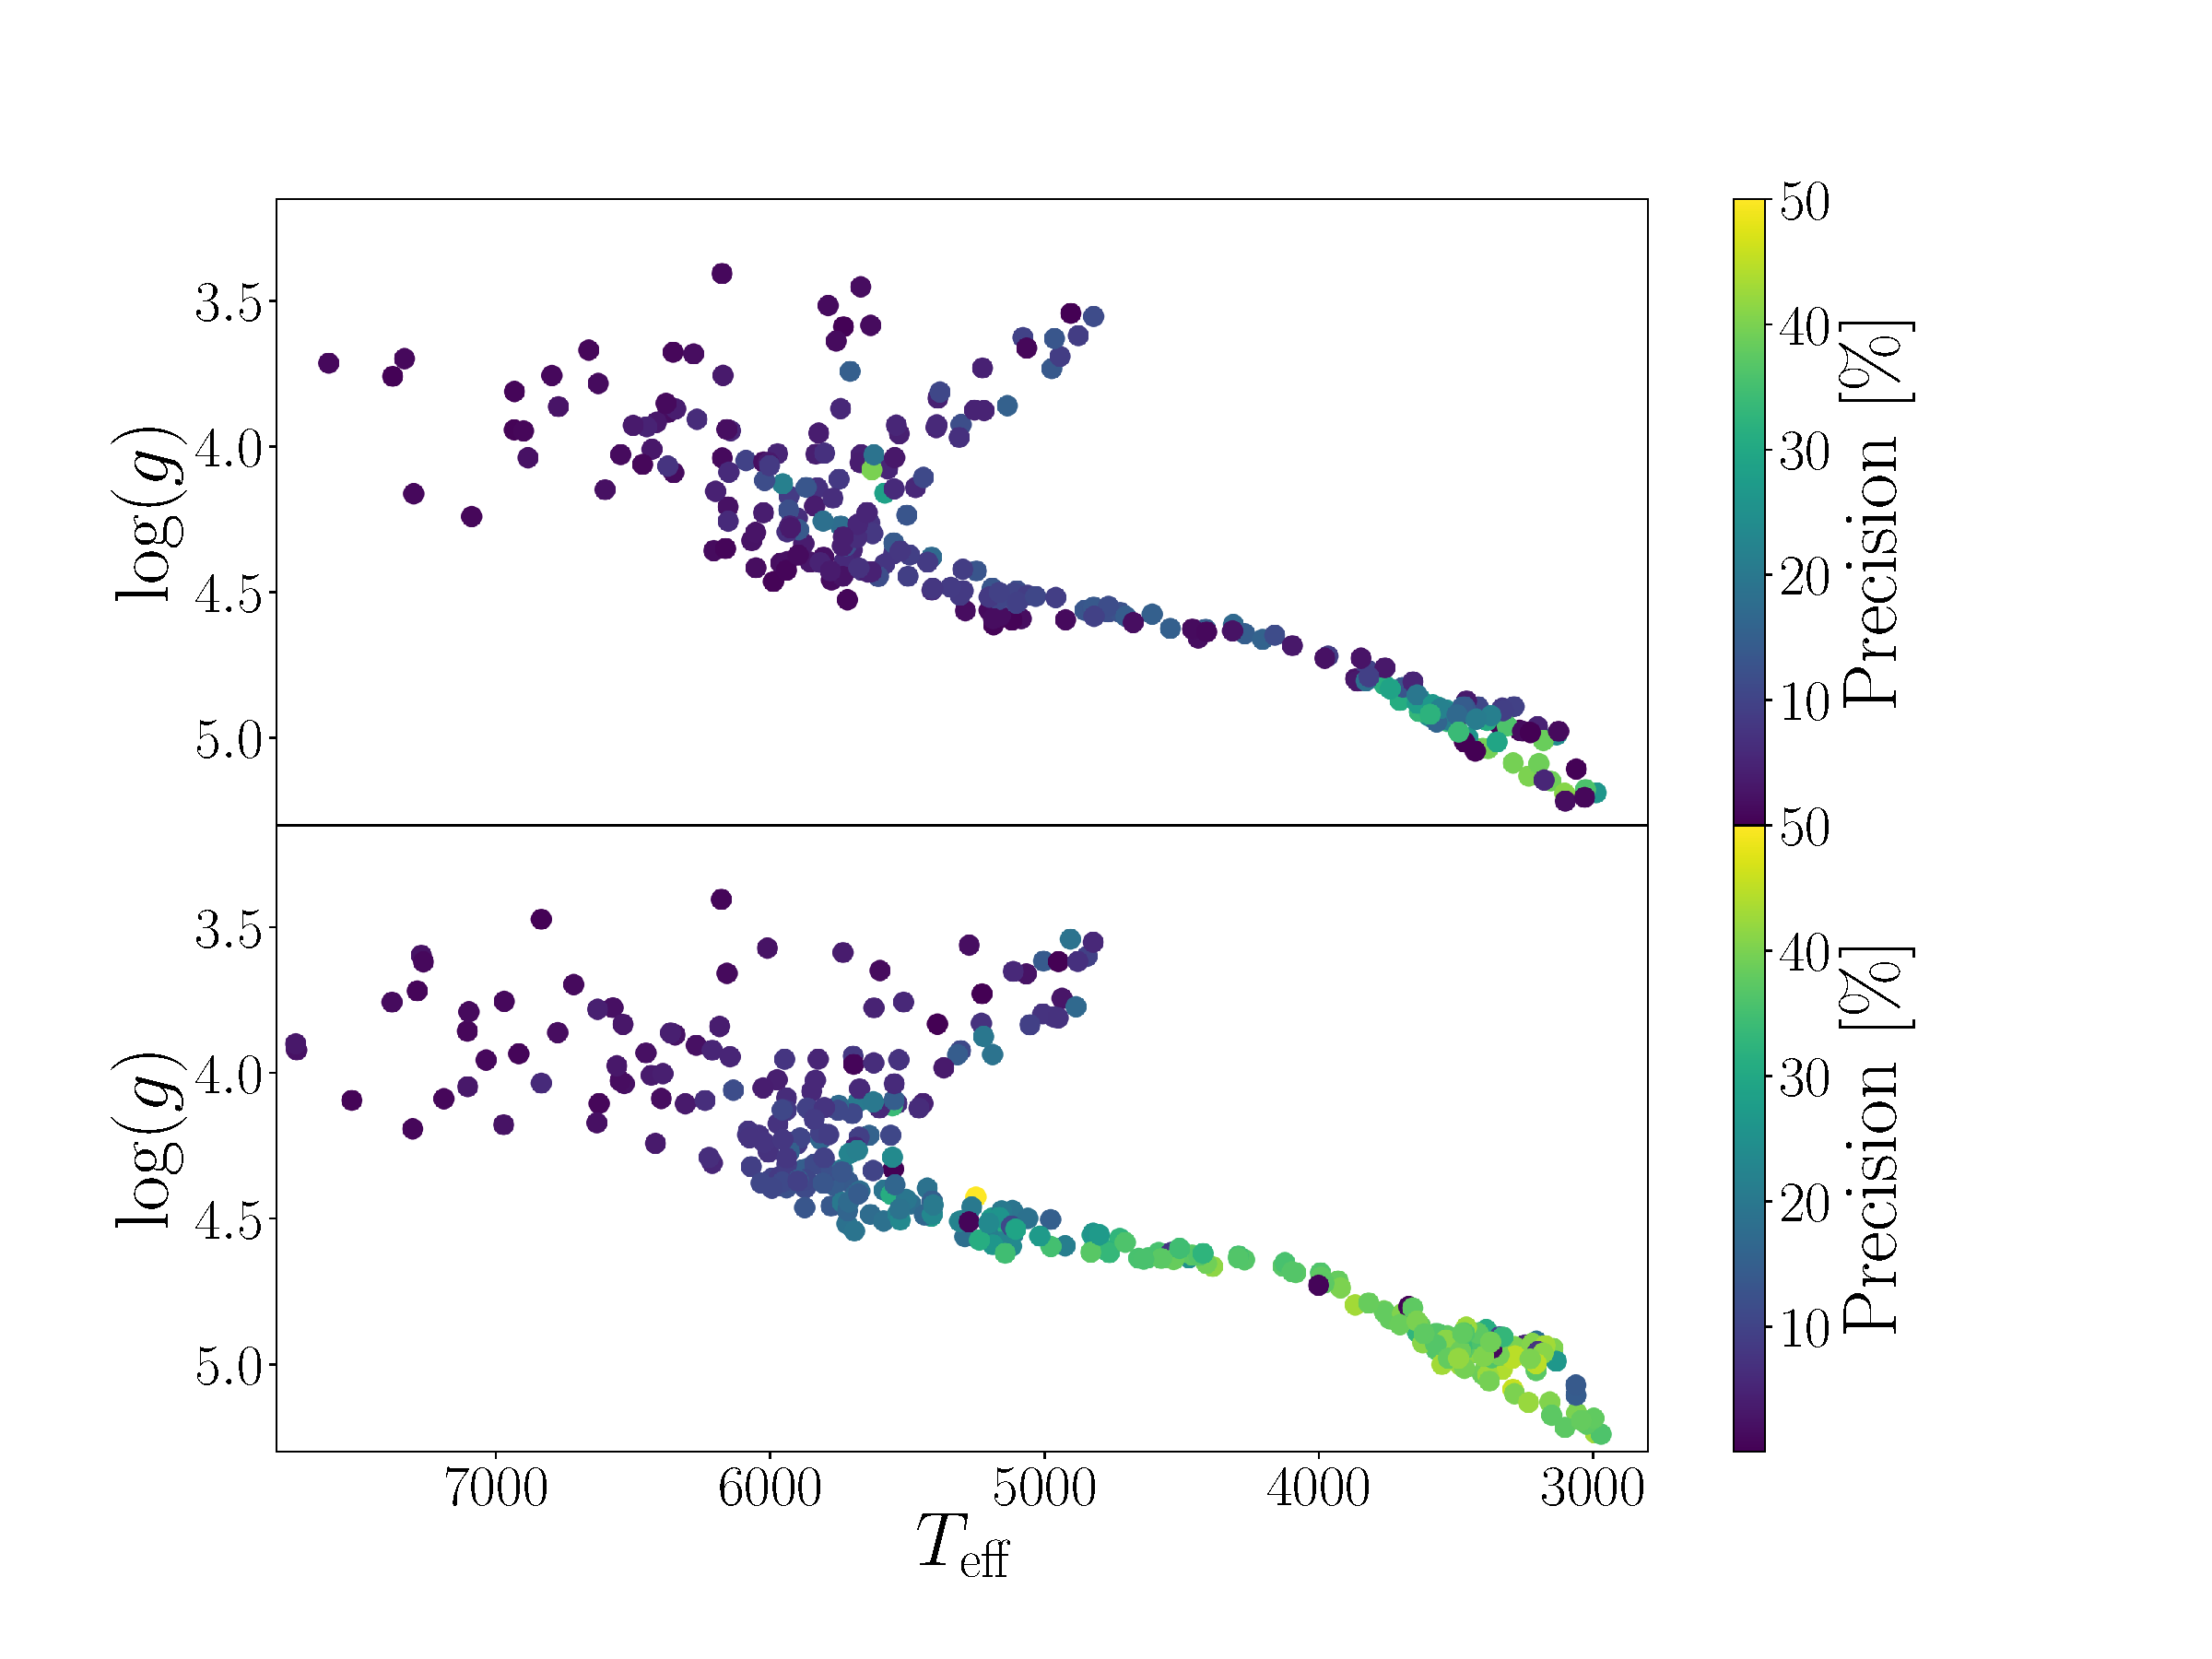
\includegraphics[width=1\textwidth]{precision_plot}
% \label{fig:precision}
% \end{figure}

This simulation experiment was designed to show the theoretical improvement in
age precision when gyrochronology is incorporated into isochrone fitting.
However, it does not demonstrate the accuracy of this method because the test
data were simulated from the same model used to infer ages.
The results of this experiment are therefore extremely accurate by design.
When applying this method to real data, the results will only be accurate if
the model is accurate.
In other words, \sd, like any age-dating method, provides model-dependent
ages.
Stellar ages calculated with \sd\ depend on both the accuracy of the MIST
models {\it and} the accuracy of the gyrochronology model (equation
\ref{eqn:gyro}).
In order to test the accuracy of \sd, we applied it to real data, as described
in the following section.

\subsection{Test 2: Open clusters}
In order to test our model on real stars with known ages, we selected a sample
of stars in the 2.5 Gyr NGC 6819 cluster.
We compiled \kepler-based rotation periods \citep{meibom2015}, \Gaia\
photometry and \gaia\ parallaxes for members of the NGC 6819 cluster.
Figure \ref{fig:NGC6819} shows the period-color relation of this
cluster and figure \ref{fig:NGC6819_results} shows the results of inferring
the ages of individual cluster members using a combination of gyrochronology
and isochrone fitting (via \sd) and isochrone fitting alone.
The ages of F stars in this cluster (\gcolor\ $\sim$ 5.5-6.5) were relatively
precisely constrained by isochrone fitting alone because, at 2.5 Gyr, they are
approaching the MS turnoff.
For these hot stars, ages inferred with gyrochronology and isochrones were
similar to ages inferred with isochrones and similarly precise, showing that
isochrones provide a lot of age information for these stars and rotation
periods do not add significantly more information.
The G and early K stars in this cluster (\gcolor\ $\lesssim$ .65) were not
precisely recovered from isochrone fitting alone -- the isochrone-only age
posteriors tend towards the prior which is a uniform distribution between 0
and 13.8 Gyrs.
The median age of stars in the cluster was 4.27 $\pm$ 0.48 Gyr when only
isochrone fitting was used.
In contrast, including gyrochronology when inferring the ages of G and K stars
in this cluster significantly improved age precision.
The median age of stars in this cluster was 2.63 $\pm$ 0.16 Gyr when ages were
inferred with a combination of isochrone fitting and gyrochronology, using the
newly calibrated Praesepe-based gyrochronology model.
The previously-calibrated \citet{angus2015} model resulted in a median stellar
age of 2.66 $\pm$ 0.21 Gyr, which is still consistent with the established
cluster age of 2.5 Gyr.
The median age of stars in the cluster using uncorrected photometry was
slightly underestimated at 1.86 $\pm$ 0.22 Gyr.
This suggests that, despite the fact that V-band extinction is marginalized
over during the inference process, correcting for extinction {\it before} ages
are estimated will reduce bias introduced by dust.

\begin{figure}
  \caption{
    The \kepler-based rotation periods of members of the 2.5 Gyr NGC 6819 open
    cluster.
    The raw \gcolor\ colors are shown in red and the dust-corrected colors are
    shown in black.
    The dashed line shows a gyrochronology model that was fit to the Praesepe
    cluster and the Sun in this work, interpolated to 2.5 Gyrs.
    The solid blue line shows a previously calibrated gyrochronology model
    \citep{angus2015}.
    This figure was generated in a Jupyter Notebook available at:
    \url{https://github.com/RuthAngus/stardate/blob/master/paper/code/NGC6819.ipynb}
  }
  \centering
    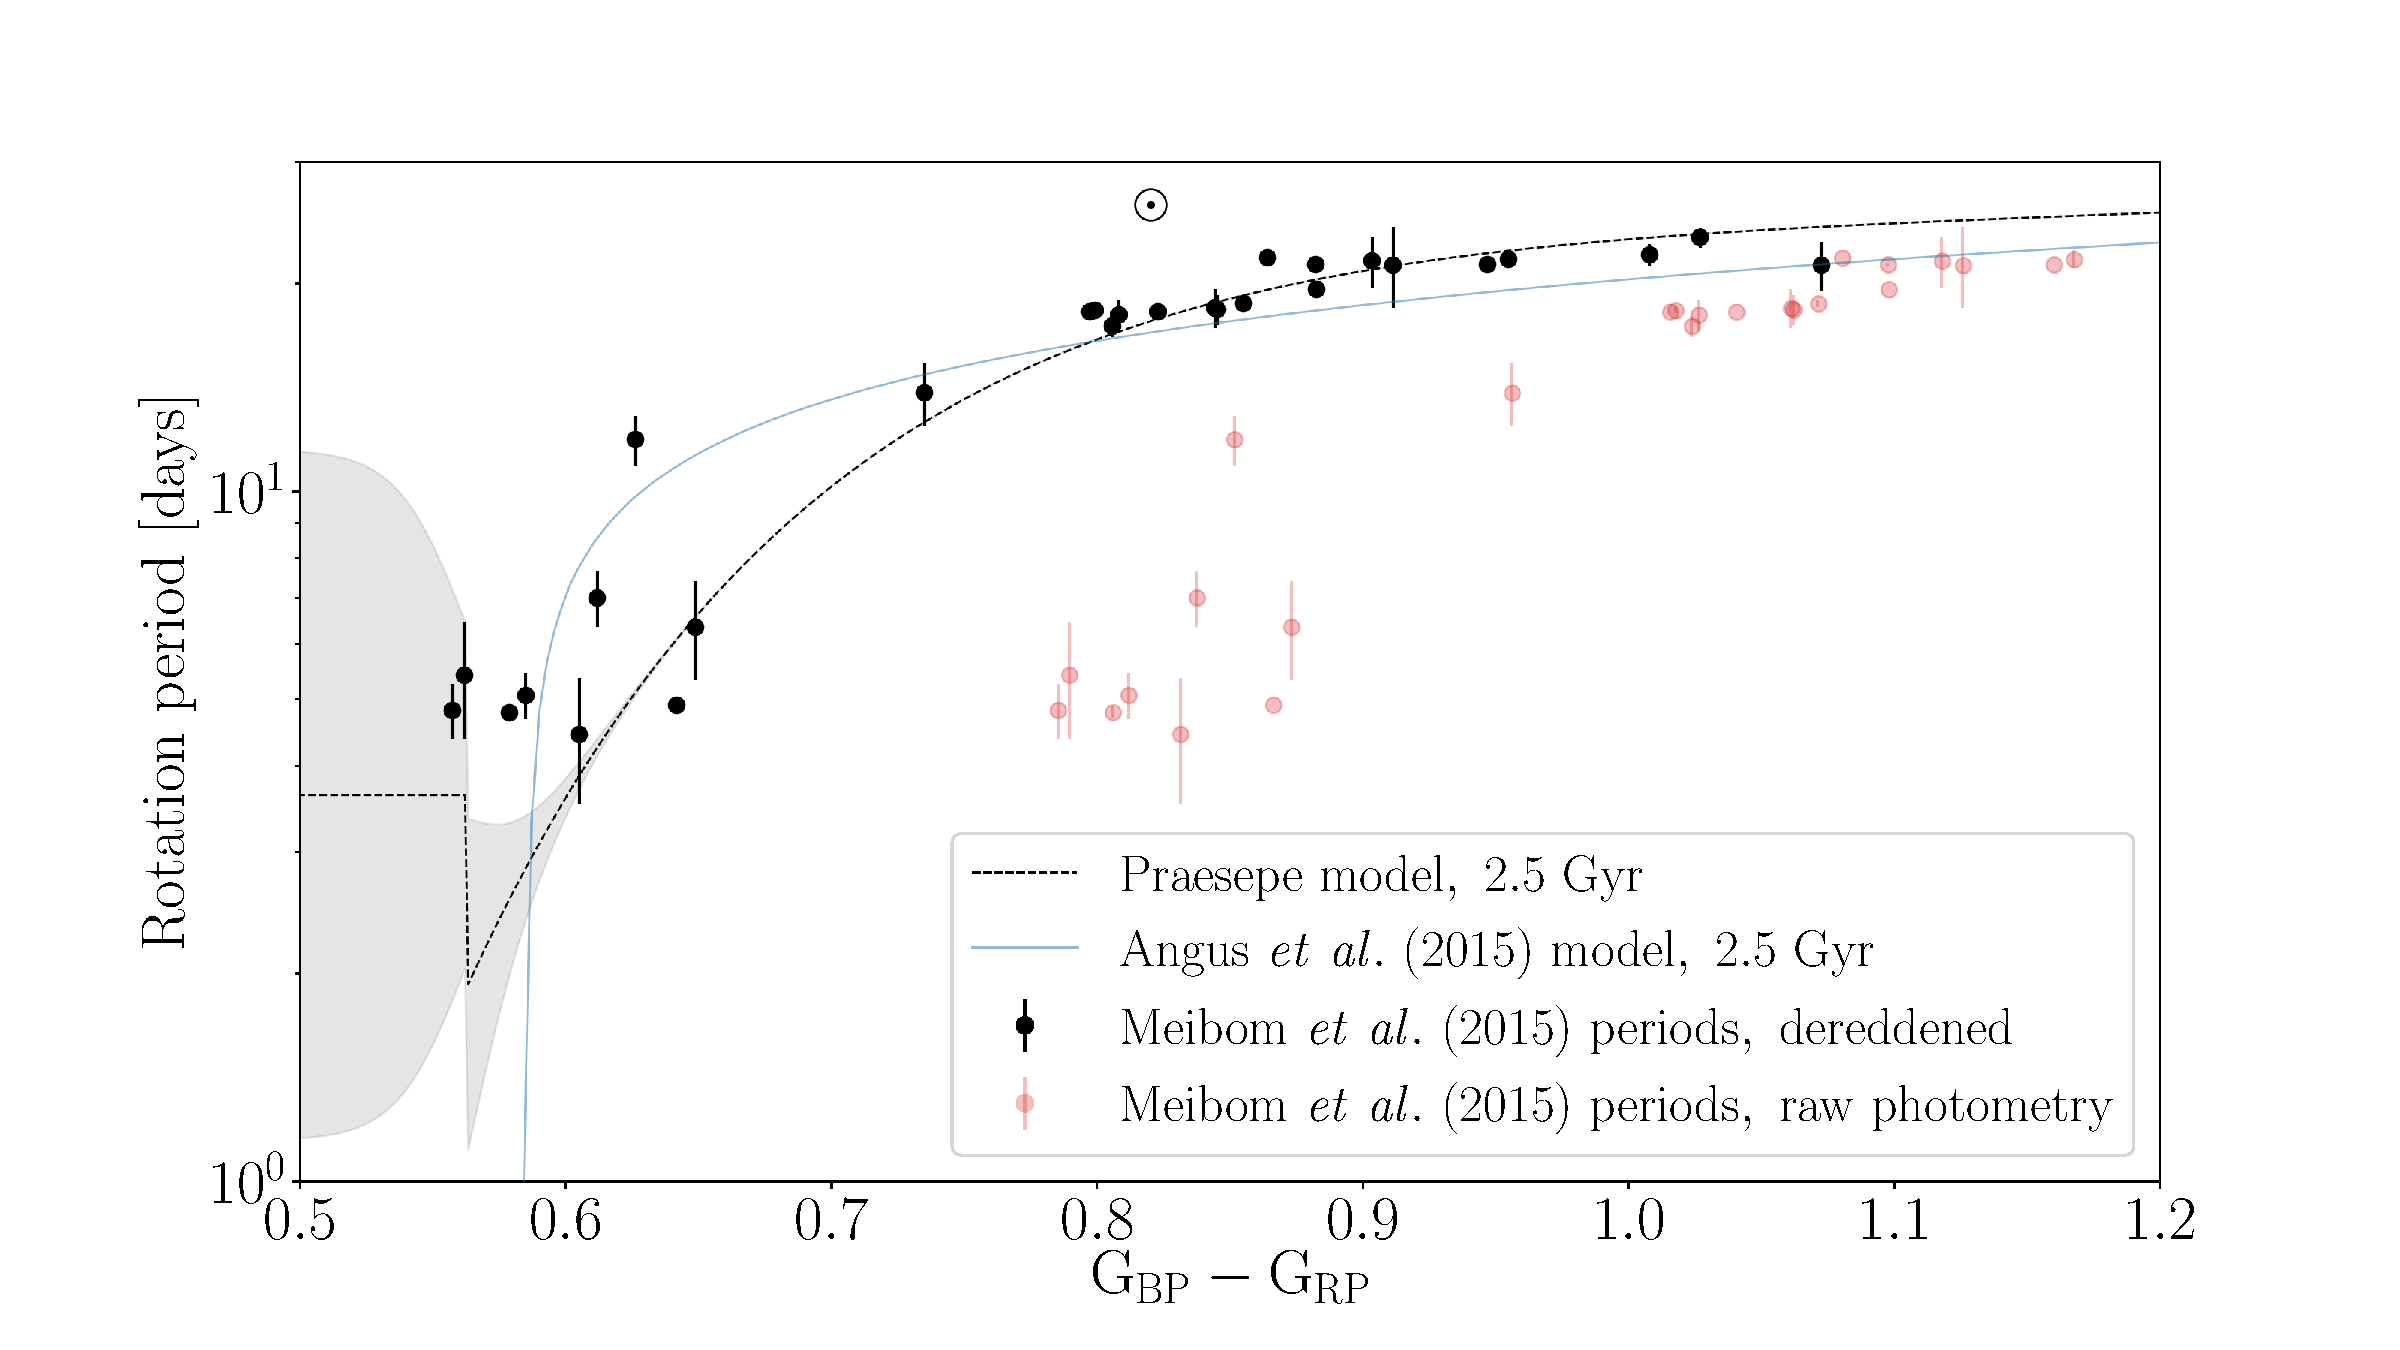
\includegraphics[width=1\textwidth]{NGC6819}
\label{fig:NGC6819}
\end{figure}

\begin{figure}
  \caption{
    The inferred ages of members of the NGC 6819 open cluster as a function of
    their \gcolor\ color.
    Ages of stars inferred using a combination of isochrone fitting and
    gyrochronology (Praesepe and Sun calibration) with dereddened \gaia\ $G$,
    $G_{BP}$, and $G_{RP}$ photometry (black circles) and uncorrected, raw,
    photometry (red squares).
    % Black circles and red squares show the ages of stars inferred using a
    % combination of isochrone fitting and gyrochronology, with a gyrochronology
    % relation that was calibrated to Praesepe and the Sun.  Black circles show
    % ages inferred with dereddened \gaia\ $G$, $G_{BP}$ and
    % $G_{RP}$ photometry and red squares show ages inferred with uncorrected,
    % raw, photometry.
    Even though V-band extinction is marginalized over in the inference
    process, reddening can still bias ages.
    Blue triangles, pointing up, show ages inferred using isochrone fitting
    and gyrochronology, with the \citet{angus2015} gyrochronology model.
    Orange triangles, pointing down, show ages inferred using isochrone
    fitting only.
    The ages of F stars (stars bluer than 0.7) were precisely constrained by
    isochrones and including gyrochronology makes little difference to their
    inferred ages.
    The age precision of G and K dwarfs (stars redder than 0.7) was improved
    by including gyrochronology.
    The median age of stars inferred using the gyrochronology model
    calibrated to Praesepe and the Sun (black circles) was 2.65 $\pm$ 0.13
    which is consistent with the established cluster age (2.5 Gyr).
    This figure was generated in a Jupyter Notebook available at:
    \url{https://github.com/RuthAngus/stardate/blob/master/paper/code/NGC6819.ipynb}
}
  \centering
    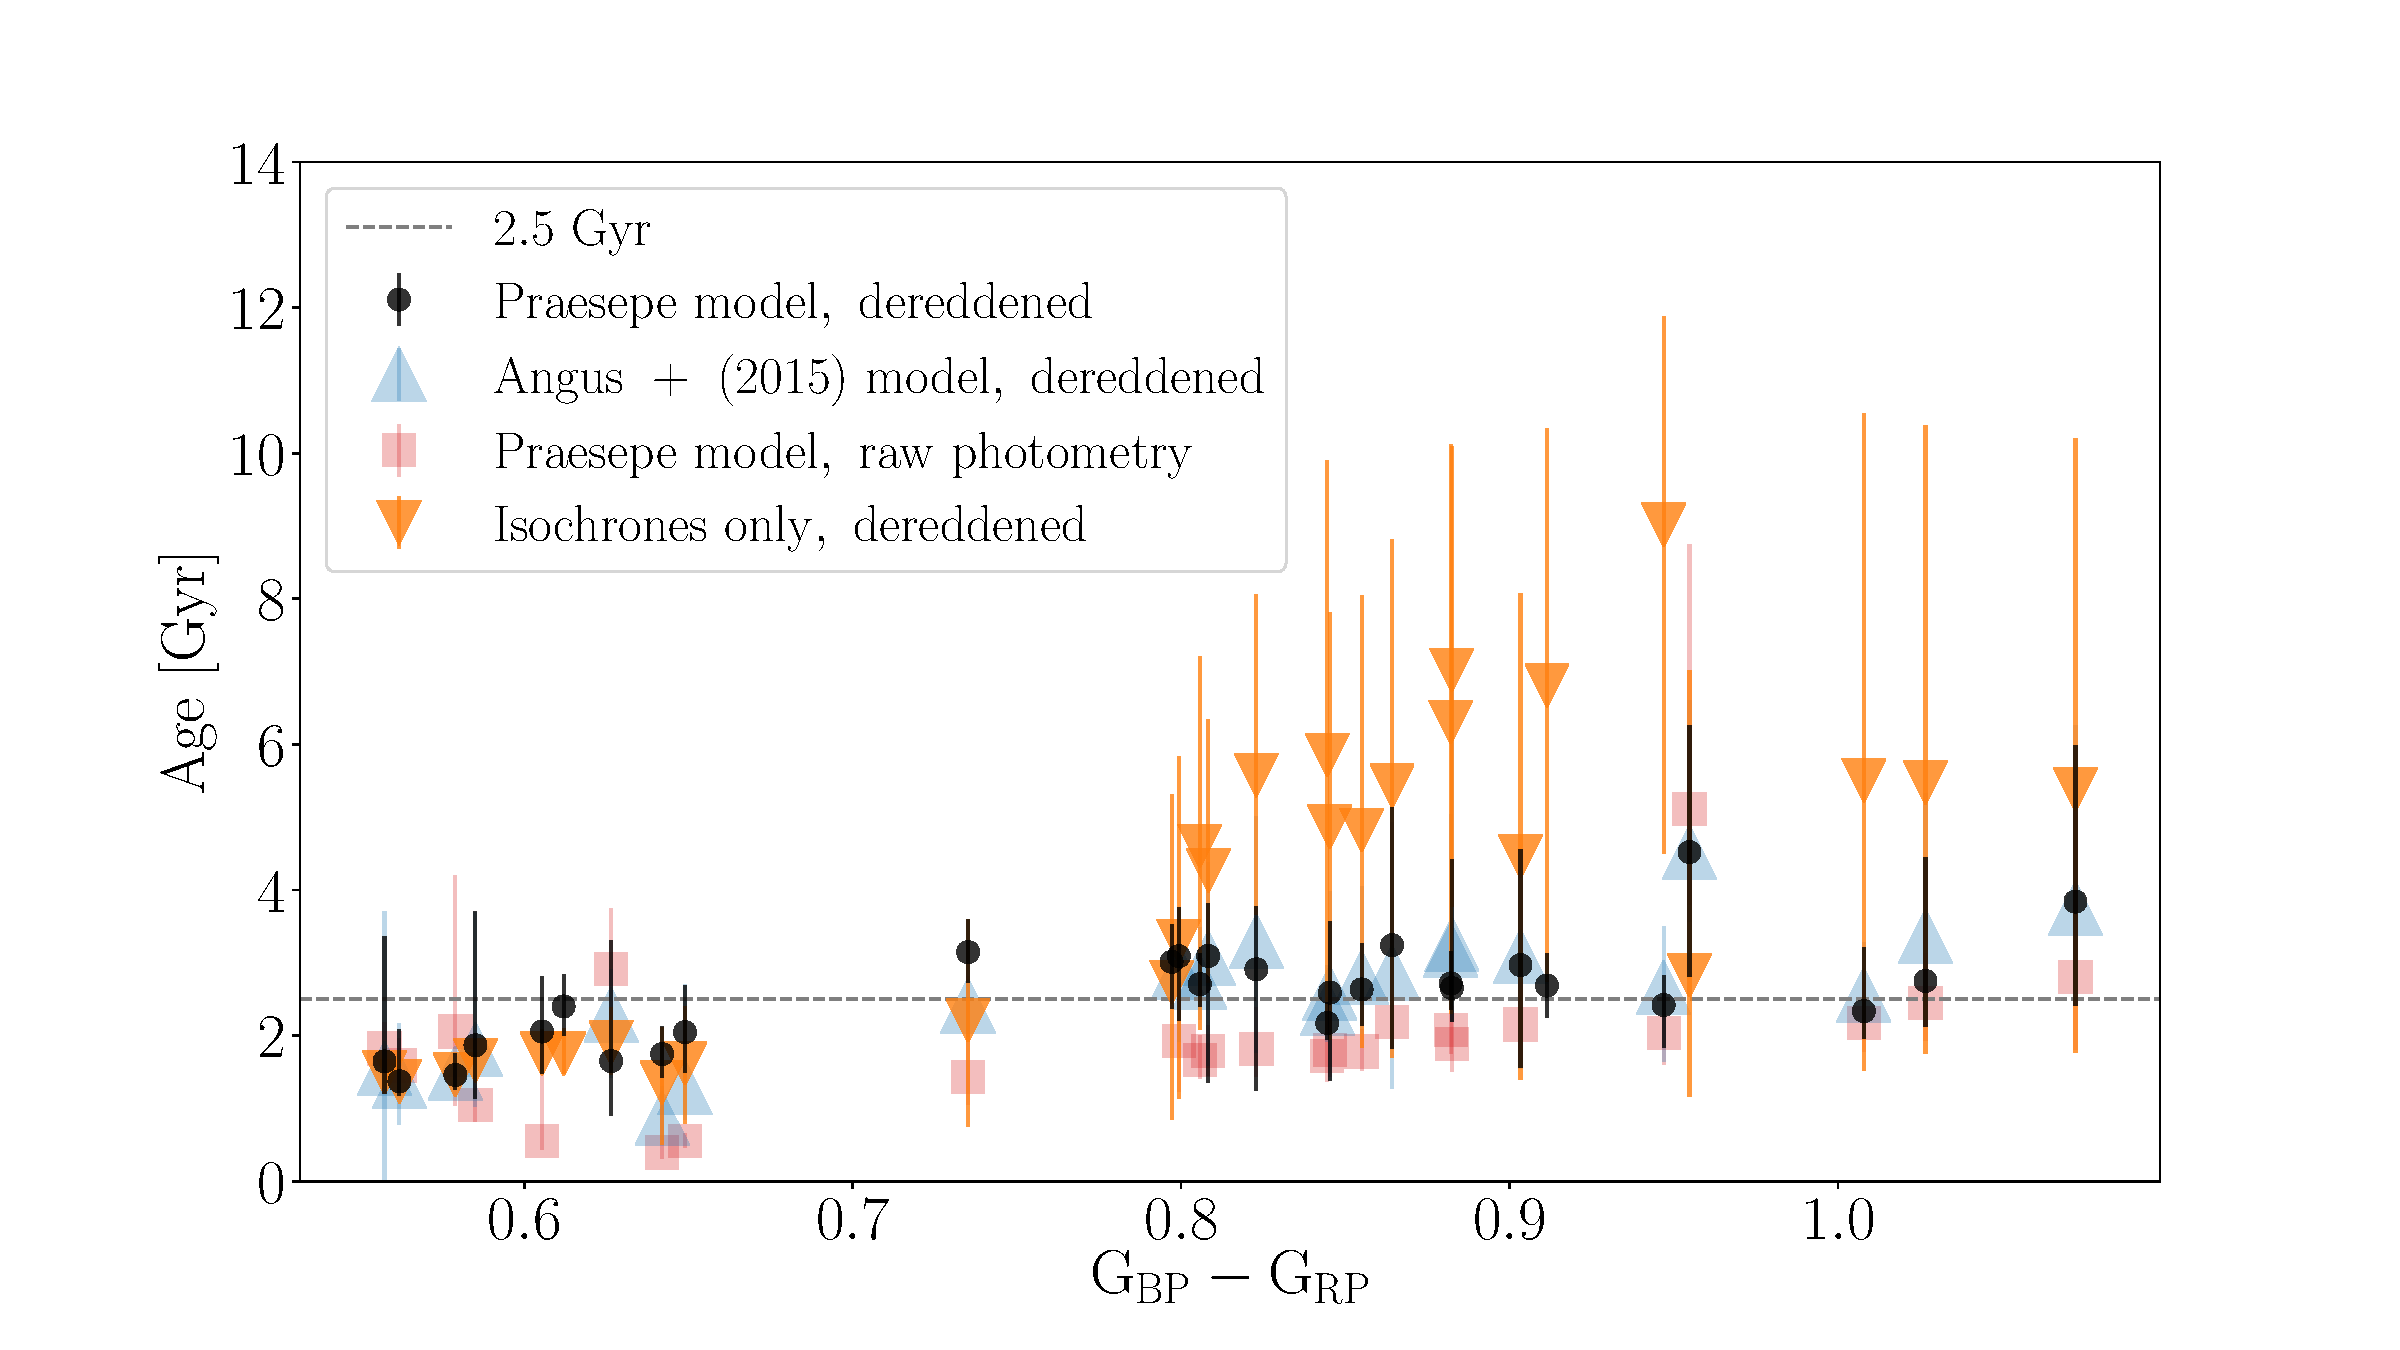
\includegraphics[width=1\textwidth]{NGC6819_results}
\label{fig:NGC6819_results}
\end{figure}

We found that 5\% rotation period uncertainties resulted in the most accurate
ages for NGC 6819.
The uncertainties on the measured rotation periods, provided in
\citet{meibom2015} and shown in figure \ref{fig:NGC6819}, were likely
underestimated for some stars.
Underestimated rotation period uncertainties can result in inaccurate age
estimates.
This raises the question: how should uncertainties on rotation periods be
estimated?
The likelihood is weighted by the inverse variance, so uncertainties on the
rotation period control the relative information provided by gyrochronology,
isochrones, and the prior.
If rotation period uncertainties are either too large or too small, the
resulting age estimate will be imprecise and/or inaccurate.
It is difficult to measure uncertainties on rotation periods directly:
standard techniques such as Lomb-Scargle periodograms and autocorrelation
functions do not provide them.
% In general, formal rotation period uncertainties should probably be calculated
% empirically via simulations as in the \citet{aigrain2015} study.
\racomment{Ideally, rotation period uncertainties should capture {\it both} the
measurement precision, {\it and} the physical uncertainty introduced by the
latitudinal movement of star spots on the surface of a differentially rotating
star.
For example, \citet{donahue1996} demonstrated that the seasonal variation in
measurements of G and K star rotation periods is a function of period, $\Delta
\mathrm{P_{rot}} \propto \mathrm{P_{rot}}^{1.3\pm0.1}$.
This variation is presumably caused by a latitudinal drift in the dominant
active regions, which traces the stellar cycle over several years, in
combination with latitudinal differential rotation.
This suggests that latitudinal spot drifting does not significantly
affect stellar rotation periods when stars are young, for example the scatter
of rotation periods about the mean gyrochronology model in Praesepe is only
around 5\%.
However it is likely that this effect will become more important at older
ages.
% The impact of this phenomenon on gyrochronology remain to be seen, and an
% in-depth study is warranted.
A thorough exploration of how rotation period uncertainties, from both
measurement uncertainty and physical variation, affect stellar ages via
gyrochronology is key to understanding the power of gyrochronology as an
age-dating method.
For now, we leave this exploration for a future study.}

\subsection{Test 3: Kepler asteroseismic stars}
\racomment{In order to test our method in the regime where both isochrone
fitting and gyrochronology become important, we recovered the ages of the 21
asteroseismic stars analysed in \citet{vansaders2016}.
These 21 stars were observed in \kepler's short cadence mode and are a mixture
of dwarfs and subgiants.
Their asteroseismic ages were calculated from the analysis of the frequencies
of individual oscillation modes \citep{mathur2012, metcalfe2014,
silvaaguirre2015, ceillier2016}, and their rotation periods from their
\kepler\ light curves \citep{garcia2014}.
We crossmatched these stars with the \Gaia\ catalog to obtain parallaxes and
apparant magnitudes in the \Gaia\ G, $\mathrm{G_{BP}}$ and $\mathrm{G_{RP}}$
band passes.
We also added J, H and K 2MASS magnitudes from the Kepler input catalog
\citep{brown2011},
% asteroseismic parameters $\Delta_\nu$ and $\nu_{\mathrm{max}}$ from
% \citet{ceillier2017} and \citet{serenelli2017},
and used spectroscopic effective temperatures, spectroscopic metallicities and
rotation periods reported in table 1 of \citet{vansaders2016}.
The \gaia\ photometry is extremely precise, and we found that artificially
inflating the uncertainties on \gaia\ apparent magnitudes by a factor of 10
substantially improved the quality of fit, both in terms of MCMC convergence
and agreement with asteroseismic age measurements.
In figure \ref{fig:astero} we show the ages of these 21 stars inferred using
isochrone fitting and gyrochronology, against their asteroseismic ages,
calculated using the Asteroseismic Modeling Portal (AMP) \citep{metcalfe2009,
metcalfe2012, metcalfe2014}.
In this figure, the colored symbols show ages inferred using a combination of
gyrochronology and isochrone fitting, implemented with the \sd\ {\it Python}
package.
The black and grey triangles show ages inferred from gyrochronology only,
where the mass and color of the stars were not inferred, but fixed to be the
asteroseismic mass and the \gaia\ \gcolor\ color.
These gyrochronal ages were calculated with age as the only free parameter,
without marginalizing over stellar mass, \gcolor\ color or extinction.
As a result, these gyrochronal ages are {\it not the same} as the ages given
by the maximum of the gyrochronal likelihood function used in the combined
age model, they simply represent an approximation to the gyrochronal age.
Grey triangles are shown for stars where gyrochronology is not applicable
because the stars are either too metal poor, too metal rich, or too evolved.
Black triangles are shown for stars where gyrochronology {\it is} applicable.
The white circles show ages inferred from isochrones only.
Dashed lines connect the three different age measurements for the same
stars.
}

\racomment{
Although the ages of all 21 stars shown in figure \ref{fig:astero} were
inferred with a joint isochronal and gyrochronal model, most (all but 8) were
either too evolved, too metal poor, or too metal rich for gyrochronology to
contribute any information to the ages.
These metal poor/rich or evolved stars lie in a regime where the variance on
their rotation period was artificially inflated because the gyrochronology
relations are not thoroughly understood or well calibrated.
The rotation periods of the remaining eight stars {\it did} contribute to
their inferred ages to some degree, however isochrones still dominated the age
information for some of them because these stars are relatively old and/or
relatively hot.
% Isochrones are information-rich for these hot and old stars, and this is
% exactly where gyrochronology is at its most information-poor.
}

\racomment{
In general, there is relatively poor agreement between the asteroseismic ages
and the ages inferred using \sd.
Much of this discrepancy is driven by differences in the isochronal ages,
which is likely attributable to differences between the MIST stellar evolution
models and those used in the AMP analysis: a combination of the Aarhus stellar
evolution code \citep[ASTEC][]{christensen-dalsgaard2008a} and the adiabatic
pulsation code \citep[ADIPLS][]{christensen-dalsgaard2008b}.
We compared non-rotating, Solar-metallicity MIST isochrones for middle-aged
stars with Solar-metallicity BaSTI isochrones \citep{pietrinferni2004,
hidalgo2018} and found that, for stars between 4 and 8 Gyrs, in the same
effective temperature range as the asteroseismic stars, the age discrepancy
between the two sets of models can be as large as 1-2 billion years.
The MIST isochrones lie above the BaSTI isochrones on the HR diagram, leading
to a systematic underprediction of ages.
}

\racomment{
The gyrochronal ages, where gyrochronology is applicable, do not show
excellent agreement with the asteroseismic ages either.
The four hot stars to the left in figure \ref{fig:astero} are rotating more
slowly than predicted by the Praesepe-based gyrochronology models, and as a
result their gyro-ages are older than their asteroseismic ones.
For these hot stars, two out of four have ages that are still consistent, or
close to consistent, with their asteroseismic ages.
The third star from the left is an anomalously slow rotator for its age and
mass and \citet{vansaders2016} also found this star to be surprisingly slowly
rotating.
In contrast, the star with a black triangle symbol (indicating that
gyrochronology is applicable) furthest to the right is {\it rapidly} rotating
for its mass and age, even when weakened braking is taken into account.
% Both stars are around Solar mass (1.06 \pm 0.02 and 1.0 \pm 0.03 M$_\odot$
% from left to right) and have asteroseismic ages older than the Sun (6.82 \pm
% 0.28 and 7.28 \pm 0.51 Gyr from left to right), and yet both rotate more
% rapidly than the Sun (23.2 \pm 7.4).
This star is around Solar mass (1.0 $\pm$ 0.03 M$_\odot$) and has an
asteroseismic age older than the Sun (7.28 $\pm$ 0.51 Gyr), yet rotates with a
period of only 19.8 $\pm$ 1.3 days.
This is KIC 9098294, a single-lined spectroscopic binary with an orbital
period of around 20 days (Latham, private communication).
It is the only clear SB1 in the \citet{vansaders2016} sample, although some
others do have binary companions with long orbital periods, for which tidal
interactions are not expected to be strong.
}

\begin{figure}
    \caption{ A comparison of stellar ages inferred using
    asteroseismic modeling with ages inferred using a combination of isochrone
    fitting and gyrochronology.
Colored circles show ages inferred using isochrone fitting and gyrochronology
combined via the \sd\ software package.
Black triangles show the ages of all stars inferred via gyrochronology only
    and white circles show ages inferred via isochrone-fitting only.
% This plot shows that, for the majority of stars in this sample, isochrone
%     fitting dominates the age information and gyrochronology only contributes
%     significantly for two or three stars.
% This is a consequence of many of these stars being hot old, extremely metal
%     rich, extremely metal poor, or evolved.
  }
  \centering
    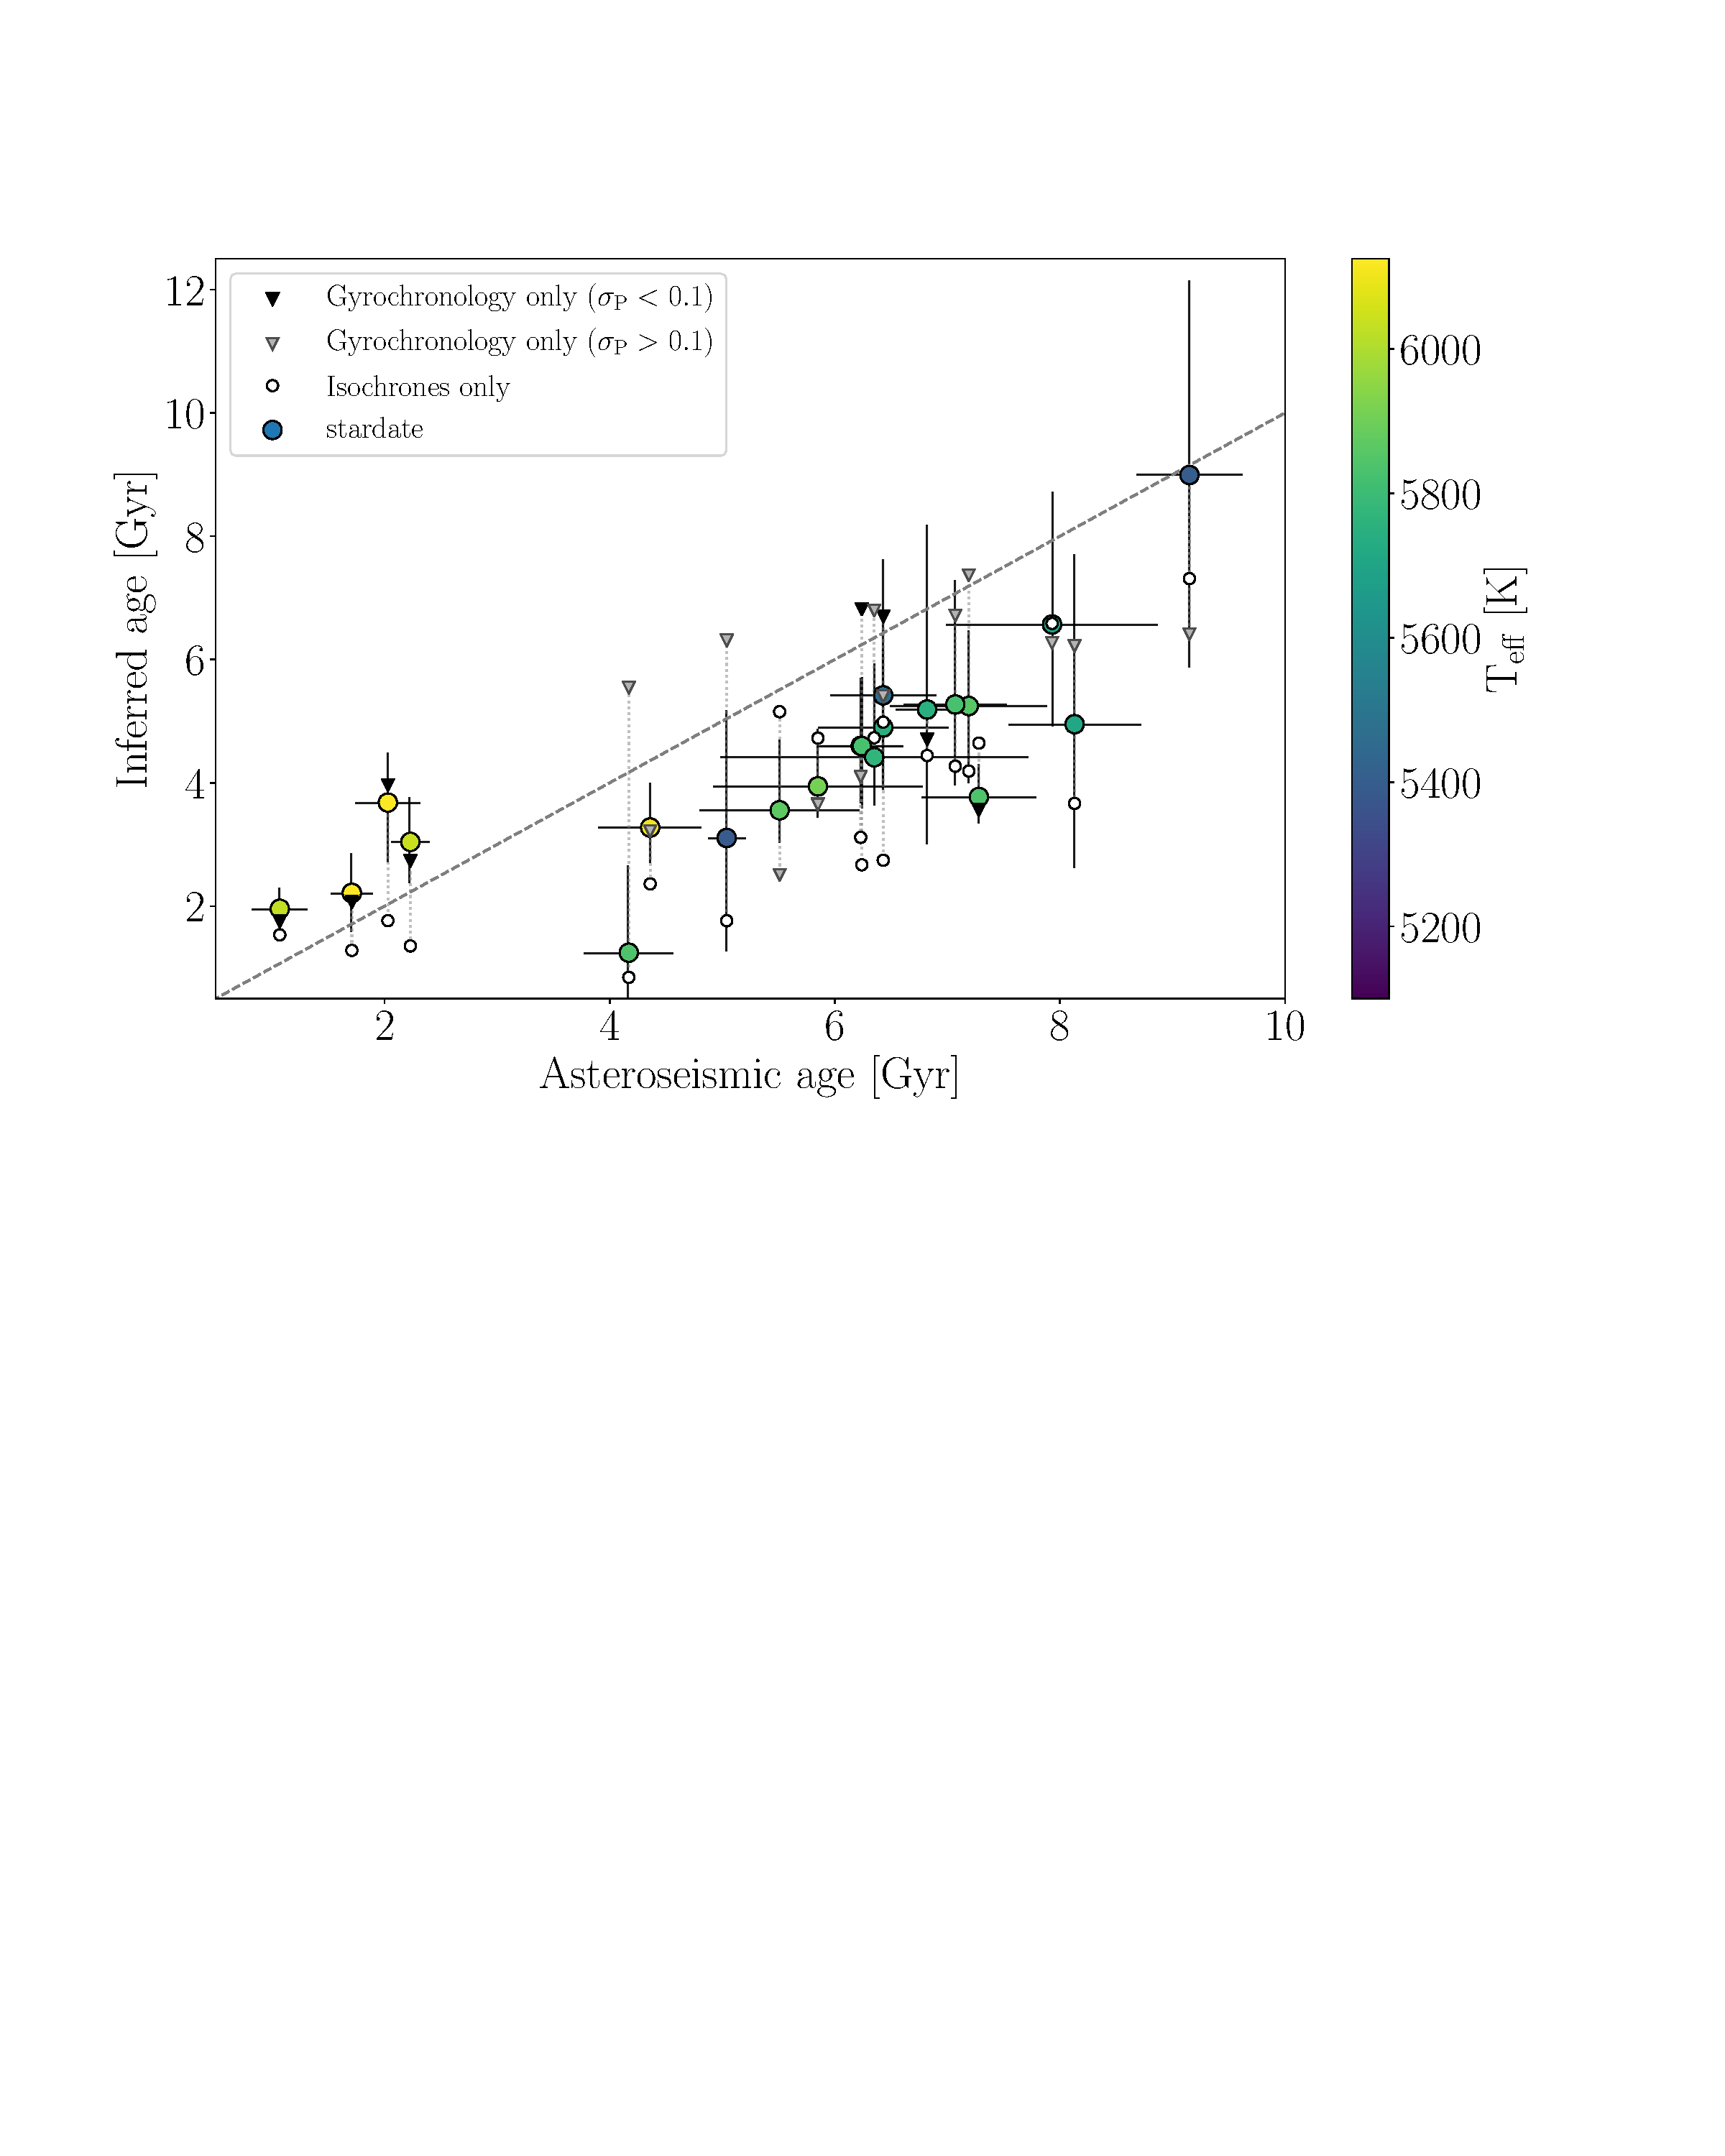
\includegraphics[width=1.2\textwidth]{asteroseismic_results_nosdss_gaia}
\label{fig:astero}
\end{figure}

\section{Conclusions}
\label{section:conclusion}

We present a statistical framework for measuring precise ages of MS stars and
subgiants by combining observables that relate, via different evolutionary
processes, to stellar age.
Specifically, we combined HRD/CMD placement with rotation periods, in a
hierarchical Bayesian model, to age-date stars based on both their hydrogen
burning and magnetic braking history.
The two methods of isochrone fitting and gyrochronology were combined by
taking the product of two likelihoods: one that contains an isochronal model
and the other a gyrochronal one.
We used the MIST stellar evolution models and computed isochronal ages and
likelihoods using the {\tt isochrones} {\it Python} package.
We fit a new broken power law gyrochronology model to the Praesepe cluster
and included a modification recommended by \citet{vansaders2016} that accounts
for weakened magnetic braking at Rossby numbers larger than 2.
The rotation periods of hot stars, cool stars, evolved stars, young stars and
metal poor and rich stars were modeled with a broad log-normal distribution.
We tested \sd\ on simulated data and cluster stars and demonstrated that
combining gyrochronology with isochrone fitting improves the precision of age
estimates for FGK dwarfs by a factor of 3 over isochrone fitting alone,
assuming 5\% measurement uncertainties on rotation periods.
Incorporating rotation periods into stellar evolution models also improves the
precision of the equivalent evolutionary phase (EEP) parameter and, since EEP,
combined with age and metallicity, determines the mass, radius and \logg\ of a
star, this means rotation periods can improve the precision of {\it all}
stellar parameters.
Although V-band extinction is marginalized over during inference, correcting
photometry for dust-extinction before analysis, or including it as a
prior can improve the accuracy of stellar ages measured with \sd.
\racomment{
We also tested \sd\ on a set of 21 \kepler\ asteroseismic stars
\citep{vansaders2016}.
We found that discrepancies between ages measured with \sd\ and ages measured
with asteroseismology are likely produced by differences between the MIST and
BaSTI stellar evolution models.
% In general, the new Praesepe-based gyrochronology relation is not a good model
% for all asteroseismic stars.
% Ultimately, these empirical gyrochronology relations need further, and
% more detailed calibration.
Asteroseismic and cluster stars provide an opportunity for calibration but
given the high-dimensionality of the gyrochronology relations (\ie\ rotation
period depends on age, mass, metallicity, surface gravity, etc), many stars
with precise ages, spanning a range of properties, are still needed to
reliably calibrate them.
}

In cases where gyrochronology predicts inaccurate stellar ages it is either
because models are not correctly calibrated, because the rotation periods or
rotation period uncertainties are themselves inaccurate, or because of
rotational outliers.
For example, \sd\ may predict inaccurate ages for stars in close binaries
whose interactions influence their rotation period evolution.
Rotational outliers are often seen in clusters \citep[see \eg][]{douglas2016,
rebull2016, douglas2017, rebull2017} and many of these fall above the main
sequence on a CMD, indicating that they are binaries.
In addition, measured rotation periods may not always be accurate and can, in
many cases, be a harmonic of the true rotation period.
For example, a common rotation period measurement failure mode is to measure
half the true rotation period.
The best way to prevent an erroneous or outlying rotation period from
resulting in an erroneous age measurement is to {\it allow} for outlying
rotation periods using a mixture model, a feature that could be built into
\sd\ in the future.

% Motivation
The optimal way to age-date stars is by combining {\it all} their available
age-related observables.
This could ultimately include activity dating via flare rates and
chromospheric activity indices, kinematic dating and chemical dating.
Of all the established age-dating methods, gyrochronology and isochrone
fitting are two of the most complementary.
The two methods are optimal in different parts of the HRD:
gyrochronology works well for FGK dwarfs and isochrone fitting works well for
subgiants and hot stars, so combining the two methods results in consistently
precise ages across a range of masses, ages and evolutionary stages.
In addition, using both methods at once circumvents the need to decide which
method to use {\it a priori}.
It eliminates the circular process of classifying a star based on its CMD
position (M dwarf, subgiant, etc), then deciding which age-dating method to
use, then inferring an age which itself depends on the classification that was
made.
It is important to infer all stellar properties at once since they all depend
on each other.
\sd\ is applicable to a large number of stars: FGKM dwarfs and subgiants with
a rotation period and broad-band photometry.
This already includes tens-of-thousands of \kepler\ and \ktwo\ stars and could
include millions more from \tess, \lsst, \wfirst, \plato, \gaia, and others in
the future.

The code used in this project is available as a {\it Python} package called
\sd, DOI: \url{ https://doi.org/10.5281/zenodo.2712419}.
It is available for download via Github\footnote{git clone
https://github.com/RuthAngus/stardate.git} or through
PyPI\footnote{pip install stardate\_code}.
Documentation is available at \url{https://stardate.readthedocs.io/en/latest/}.
All code used to produce the figures in this paper is available at
\url{https://github.com/RuthAngus/stardate}.
This paper is based on code with the following Git hash:
f739562c1546e117e9bb217e1732c62b41be8061.
% git log --pretty=format:'%H' -n 1
% git log --pretty=format:'%h' -n 1

Some of the data presented in this paper were obtained from the Mikulski
Archive for Space Telescopes (MAST).
STScI is operated by the Association of Universities for Research in
Astronomy, Inc., under NASA contract NAS5-26555.
Support for MAST for non-HST data is provided by the NASA Office of Space
Science via grant NNX09AF08G and by other grants and contracts.
This paper includes data collected by the Kepler mission. Funding for the
\Kepler\ mission is provided by the NASA Science Mission directorate.

This work made use of the gaia-kepler.fun crossmatch database created by Megan
Bedell

This work has made use of data from the European Space Agency (ESA) mission
{\it Gaia} (\url{https://www.cosmos.esa.int/gaia}), processed by the {\it Gaia}
Data Processing and Analysis Consortium (DPAC,
\url{https://www.cosmos.esa.int/web/gaia/dpac/consortium}). Funding for the DPAC
has been provided by national institutions, in particular the institutions
participating in the {\it Gaia} Multilateral Agreement.

This research was supported in part by the National Science Foundation under
Grant No. NSF PHY-1748958.

% \software{Astropy \citep{http://dx.doi.org/10.1051/0004-6361/201322068},
%           Matplotlib \citep{http://dx.doi.org/10.1109/MCSE.2007.55}},
% }

\section{Appendix}
\label{section:appendix}

\subsection*{Priors}
\label{section:priors}

We used the default priors in the {\tt isochrones.py} {\it python} package.
The prior over age was,
\begin{equation}
p(A) = \frac{\log(10) 10^{A}}{10^{10.5} - 10^8}, ~~~ 8 < A < 10.5.
\end{equation}
% where $A$, is $\log_{10}(\frac{\mathrm{Age}}{\mathrm{yrs}})$.
where $A$, is $\log_{10}(\mathrm{Age~[yrs]})$.
% The prior over mass is uniform in natural-log between -20 and 20,
% \begin{equation}
%     p(M) = U(-20, 20)
% \end{equation}
% % where $M$ is $\ln(\frac{\mathrm{mass}}{M_\odot})$.
% where $M$ is $\ln(\mathrm{Mass}~[M_\odot])$.
The prior over EEP was uniform with an upper limit of 800.
We found that adding this upper limit reduced some multi-modality caused by
the giant branch and resulted in better performance.
The prior over true bulk metallicity was based on the galactic metallicity
distribution, as inferred using data from the Sloan Digital Sky Survey
\citep{casagrande2011}.
% It is based on two double-Gaussian distribution, where the halo is described as
% a broad Gaussian and the galactic disc as a narrow Gaussian.
It is the product of a Gaussian that describes the metallicity distribution
over halo stars and two Gaussians that describe the metallicity distribution
in the thin and thick disks:
\begin{eqnarray}
    p(F) =
    & H_F \frac{1}{\sqrt{2\pi\sigma_{\mathrm{halo}}^2}}
    \exp\left(-\frac{(F-\mu_{\mathrm{halo}})^2}{2\sigma_{\mathrm{halo}}}\right)
    \\ \nonumber
    & \times (1-H_F)
    \frac{1}{\xi}
    \left[\frac{0.8}{0.15}\exp\left(-\frac{(F-0.016)^2}{2\times 0.15^2}\right)
    + \frac{0.2}{0.22}\exp\left(-\frac{(F-0.15)^2}{2\times
    0.22^2}\right)\right],
\end{eqnarray}
where $H_F = 0.001$ is the halo fraction, $\mu_\mathrm{halo}$ and
$\sigma_{\mathrm{halo}}$ are the mean and standard deviation of a Gaussian
that describes a probability distribution over metallicity in the halo, and
take values -1.5 and 0.4 respectively.
% $\mu_\mathrm{disk, 1}$, $\mu_\mathrm{disk, 2}$, $\sigma_\mathrm{disk, 1}$
% and $\sigma_\mathrm{disk, 2}$ are the means and standard deviations of two
The two Gaussians inside the square brackets describe probability
distributions over metallicity in the thin and thick disks.
The values of the means and standard deviations in these Gaussians are from
\citet{casagrande2011}.
$\xi$ is the integral of everything in the square brackets from $-\infty$ to
$\infty$ and takes the value $\sim 2.507$.
% D_F = 0.8 \sigma_{\mathrm{disk, 1}} = 0.15 \mu_{\mathrm{disk, 1}} = 0.016
% \sigma_{\mathrm{disk, 2}} = 0.22 \mu_{\mathrm{disk, 2}} = 0.15
The prior over distance was,
\begin{equation}
    p(D) = \frac{3}{3000^3} D^2, ~~~ 0 < D < 3000,
\end{equation}
with D in kiloparsecs, and, finally, the prior over extinction was uniform
between zero and one,
\begin{equation}
    p(A_V) = U(0, 1).
\end{equation}

\bibliographystyle{plainnat}
\bibliography{hz.bib}
\end{document}
